\documentclass[twoside, 11pt]{article}
% ========== Packages ==========
\usepackage[a4paper,
  left=25mm,
  right=25mm,
  top=30mm,
  bottom=35mm,
  headheight=35mm
]{geometry}

\usepackage[ngerman]{babel} %Ändert die Sprache
\usepackage[T1]{fontenc} %Wichtig für ä ö ü
\usepackage{amssymb} %Für mathematische Zeichen
\usepackage{amsthm} %Für mathematische Umgebungen
\usepackage{graphicx}
\usepackage{fancyhdr}
\usepackage[utf8]{inputenc}
\usepackage{multirow} %Für Tabellen
\usepackage{longtable} %Für lange Tabellen
\usepackage{tabularx}
\usepackage{pdfpages} %Zum einfügen von PDF's
\usepackage{hyperref} %Für hyperlinks
\hypersetup{bookmarks=true}
\usepackage{parskip}
\usepackage{caption} %Für die Beschriftung von Bilder
\captionsetup{justification=centering}
\captionsetup{font=it}
\setlength{\parindent}{0pt}
\usepackage{subcaption} %Für die Beschriftung unterteilter Bilder
\usepackage{float}
\floatstyle{plaintop}
\restylefloat{table}

\makeatletter %Für römische Zahlen
\newcommand*{\rom}[1]{\expandafter\@slowromancap\romannumeral #1@}

%Für die dicken Linien in Tabellen
\def\thickhline{%
  \noalign{\ifnum0=`}\fi\hrule \@height \thickarrayrulewidth \futurelet
   \reserved@a\@xthickhline}
\def\@xthickhline{\ifx\reserved@a\thickhline
               \vskip\doublerulesep
               \vskip-\thickarrayrulewidth
               \fi
      \ifnum0=`{\fi}}
\makeatother
\newlength{\thickarrayrulewidth}
\setlength{\thickarrayrulewidth}{2\arrayrulewidth}

%Sorgt dafür, dass nicht immer alles auf die ganze Seite verteilt wird.
\raggedbottom

% ========== Header and Footer ==========
\pagestyle{fancy}
\fancyhf{}
\fancyhead[RE,LO]{Seite \thepage}
\fancyhead[LE,RO]{\nouppercase{\leftmark}}
\fancyfoot[RE,LO]{BAT FS21}

%Eigens erstellte Variablen
\newcommand{\plotWidth}{0.7}
\newcommand{\garphWidth}{0.7}

% % \nomenclature{$c$}{Speed of light in a vacuum inertial system \nomunit{$299,792,458\, m/s$}}

% makeindex main.nlo -s nomencl.ist -o main.nls
\nomenclature{$N$}{The number of angels per needle point}%
\nomenclature{$B$}{The area of the needle point}%

\nomenclature{$t_k$}{Höhe des Schaumkernes}
\nomenclature{$E_k$}{E-Modul der Kernschicht}
\nomenclature{$G_k$}{Schub-Modul des Schaumkernes}
\nomenclature{$t_d$}{Höhe der Deckschicht}
\nomenclature{$E_d$}{E-Modul der Deckschicht}
\nomenclature{$h$}{Abstand der neutralen Fasern der Deckschichten}
\nomenclature{$w_b$}{Verformung durch Biegegelastung}
\nomenclature{$w_s$}{Verformung durch Schubbelastung}
\nomenclature{$w_{Ges}$}{Gesammtverformung}

\nomenclature{$P_kB$}{Euler-Knicklast des schubsteifen Balkens}
\nomenclature{$P_kS$}{Schubknicklast}
\nomenclature{$P_k$}{Kritische Knicklast}

\nomenclature{$n$}{Normalkraft pro Länge \nomunit{$N/mm$}}
\nomenclature{$m$}{Moment pro Länge \nomunit{$N$}}
\nomenclature{$q$}{Schubkraft Pro Länge \nomunit{$N/mm$}}

\nomenclature{$p$}{Streckenlast \nomunit{$N/mm^2$}}



\usepackage{nomencl}
\makenomenclature
\begin{document}
% ==================== Titelseite ====================
  \begin{titlepage}
    \begin{center}
        % \vspace*{1cm}

        \LARGE
        Bachelor-Thesis an der Hochschule Luzern\\
        Technik \& Architektur

        \vspace{0.8cm}
        \Huge
        \textbf{Solar Butterfly - Auslegung Grundstruktur}

        \vspace{3cm}

        \begin{center}
          \makebox[\textwidth]{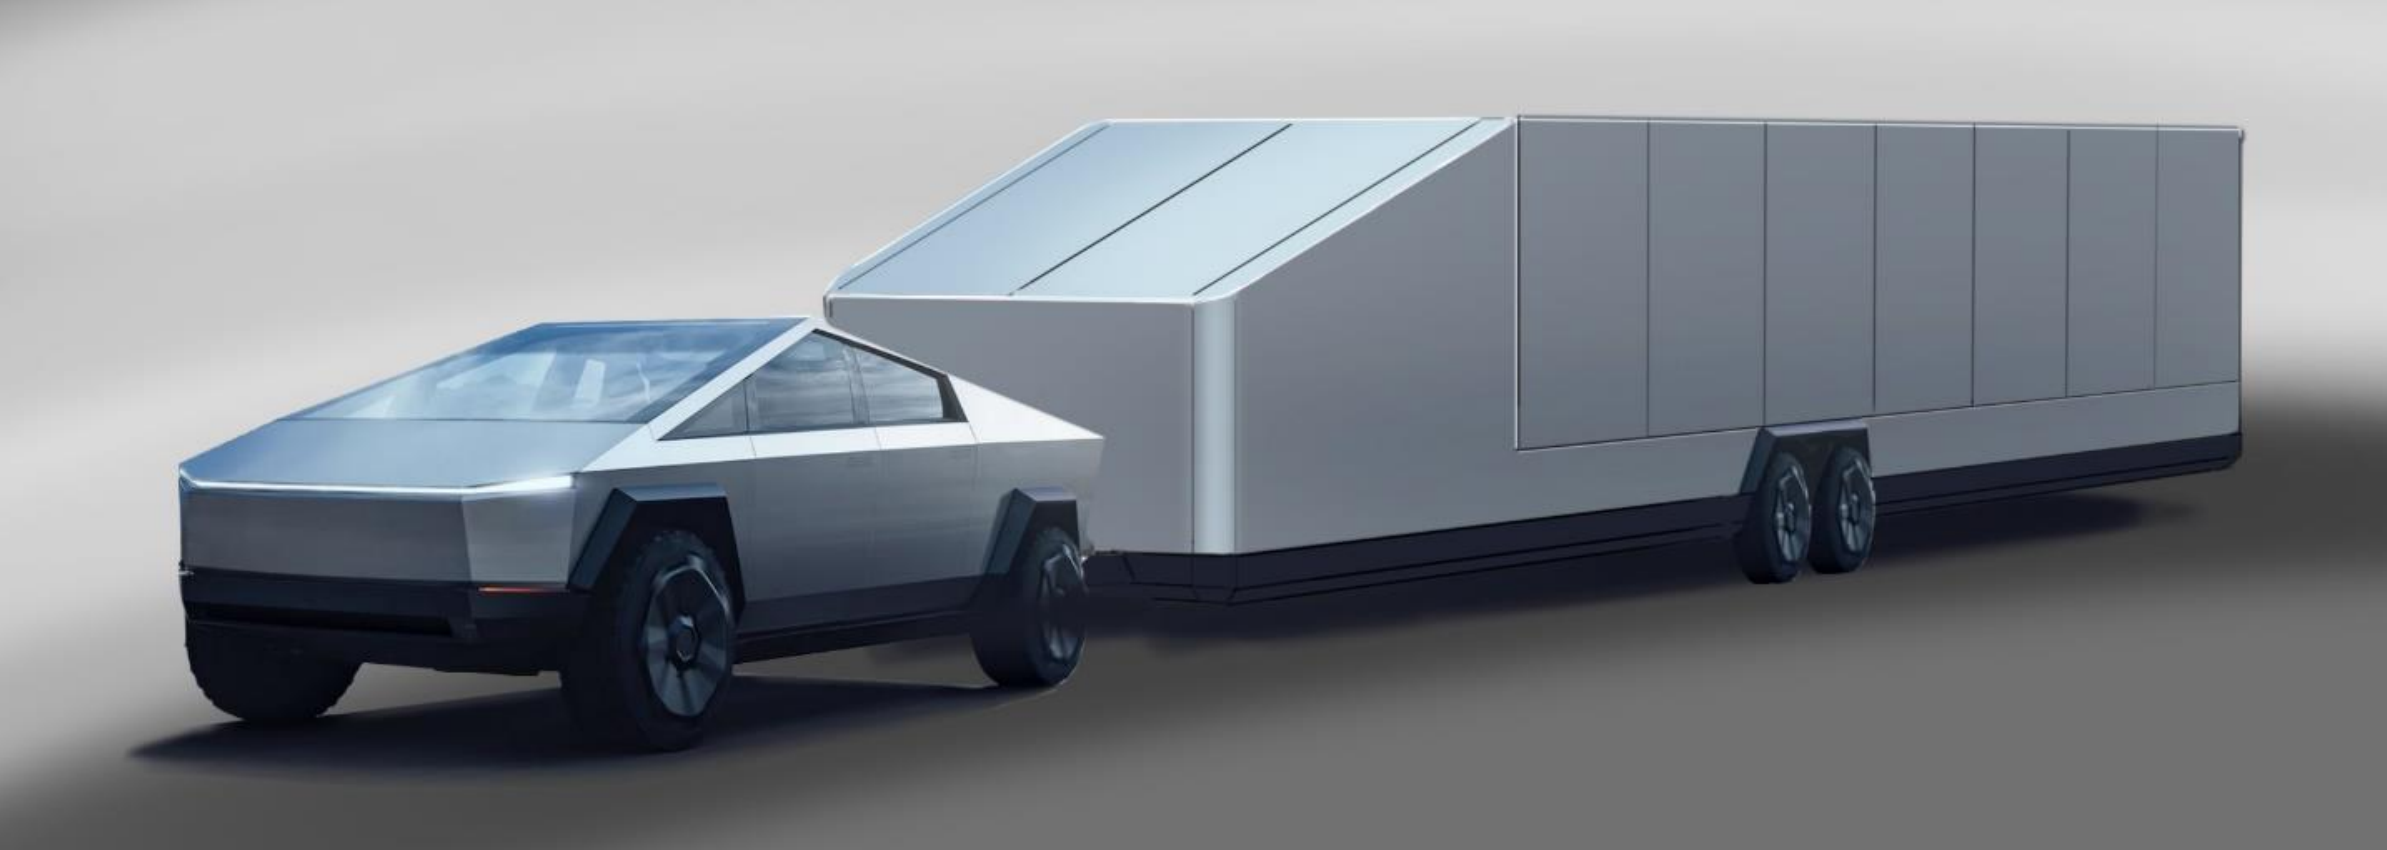
\includegraphics[width=1\paperwidth]{04_Figures/SB0.png}}
        \end{center}

        \vfill
        \begin{table}[b]
        \small
          \begin{tabularx}{\linewidth}{llX}
            \textbf{Diplomandin/Diplomand} & \textbf{Gut, Andre}                                &\\[4 mm]
            \textbf{Bachelor-Studiengang}  & \textbf{Bachelor Maschinentechnik}                 &\\[4 mm]
            \textbf{Semester}              & \textbf{FS21}                                      &\\[4 mm]
            \textbf{Dozentin/Dozent}       & \textbf{Roman\v{c}uk, Dejan}                       &\\[4 mm]
            \textbf{Expertin/Experte}      & \textbf{Dubach, Roger}                             &
          \end{tabularx}
        \end{table}

    \end{center}
\end{titlepage}


% ==================== Frontmatter ====================
  \pagenumbering{roman}
  \setcounter{page}{2}
  \vspace{2cm}
\begin{large}
\textbf{Bachelor-Thesis an der Hochschule Luzern - Technik \& Architektur}\\
\end{large}
\vspace{1cm}

\begin{table}[H]
\small
  \begin{tabularx}{\linewidth}{llX}
    \textbf{Titel}                 & \textbf{Solar Butterfly - Auslegung Grundstruktur} &\\[4 mm]
    \textbf{Diplomandin/Diplomand} & \textbf{Gut, Andre}                                &\\[4 mm]
    \textbf{Bachelor-Studiengang}  & \textbf{Bachelor Maschinentechnik}                 &\\[4 mm]
    \textbf{Semester}              & \textbf{FS21}                                      &\\[4 mm]
    \textbf{Dozentin/Dozent}       & \textbf{Roman\v{c}uk, Dejan}                       &\\[4 mm]
    \textbf{Expertin/Experte}      & \textbf{Dubach, Roger}                             &
  \end{tabularx}
\end{table}

\vspace{1.5cm}
\textbf{Abstract Deutsch}\\
Ziel des Projektes \emph{Solar Butterfly} ist die Entwicklung eines autarken Wohnwagens, welcher sich mit selbst erzeugten Solarstrom versorgen und autonom operiert werden kann. Der Solar Butterfly soll international Aufmerksamkeit erregen und so nachhaltige Lösungen im Bereich des Klimaschutzes und Elektromobilität ermutigen und vorantreiben. In Zusammenarbeit mit drei weiteren Maschinenbaustudenten und deren Bachelorarbeiten soll die Vision des Solar Butterflys in die Realität umgesetzt werden.\\
Diese Arbeit befasst sich mit dem Definieren der Anforderungen und Auslegungskriterien des Solar Butterflys, dem Bestimmen von Design-Allowables, der Ausarbeitung eines Lastenheftes und der Grobauslegung der Grundstruktur. Zur Bestimmung von Schnittgrössen soll dabei ein globales FEM-Modell zur Anwendung kommen.\\
Handrechnungen und FEM-Berechnungen zeigen, dass von den untersuchten Belastungen die Lastfälle der vertikalen und rotatorischen Beschleunigung, welche während der Fahrt auftreten, die grössten Beanspruchungen darstellen. Zugleich weisen diese Lastfälle aufgrund von nur bedingt abschätzbaren Randbedingungen die grössten Unsicherheiten und Risiken auf. Weiter konnte in Erfahrung gebracht werden, dass die Klebeverbindung zwischen dem Boden und Chassis als Kritisch zu beurteilen ist und dass weitere Untersuchungen und Abklärungen diesbezüglich nötig sind.
Ferner konnte Potential zur Gewichtsreduktion in Form einer Optimierung des Chassis in Verbindung mit dem Boden ausfindig gemacht werden.


\textbf{Abstract Englisch}\\
The goal of the project \emph{Solar Butterfly} is the development of a self-sufficient caravan, which can be powered by self-generated solar electricity and operate autonomously. The Solar Butterfly is intended to attract international attention and thus encourage and promote sustainable solutions in the field of climate protection and electromobility. In collaboration with three
other mechanical engineering students and their bachelor thesis, the vision of the Solar Butterfly is to be turned into reality.
This work deals with the definition of the requirements and design criteria for the Solar Butterfly, the specification of design allowables, the elaboration of a specification sheet and the rough design of the basic structure. A global FEM model will be used to determine the sectional forces.
Hand calculations and FEM calculations show that of the loads investigated, the load cases of vertical and rotational acceleration, which occur during driving, represent the greatest stresses. It was also found that the adhesive bond between the floor and the chassis is critical and that further investigations and clarifications are necessary. Furthermore, potential for weight reduction could be identified by optimizing the chassis in conjunction with the floor.

\vspace{2cm}
Ort, Datum $\;\;\;\;\;\;\;\;\;\;\;\;\;\;\;\;\;\;\;\;$ Luzern, 11. Juni 2021\\
\textbf{{\small $^\copyright$} Andre Gut, Hochschule Luzern - Technik \& Architektur}

\vspace*{\fill}

\noindent
{\color{gray} \rule{\linewidth}{0.5px} }
\begin{footnotesize}
  \textcolor{gray}{Alle Rechte vorbehalten. Die Arbeit oder Teile davon dürfen ohne schriftliche Genehmigung der Rechteinhaber weder in irgendeiner Form reproduziert noch elektronisch gespeichert, verarbeitet, vervielfältigt oder verbreitet werden.}\\
  \textcolor{gray}{Sofern die Arbeit auf der Website der Hochschule Luzern online veröffentlicht wird, können abweichende Nutzungsbedingungen unter Creative-Commons-Lizenzen gelten. Massgebend ist in diesem Fall die auf der Website angezeigte Creative-Commons-Lizenz.}
\end{footnotesize}
\newpage

  \textbf{Abstract Deutsch}\\
Ziel des Projektes \emph{Solar Butterfly} ist die Entwicklung eines autarken Wohnwagens, welcher sich mit selbst erzeugten Solarstrom versorgen und autonom operiert werden kann. Der Solar Butterfly soll international Aufmerksamkeit erregen und so nachhaltige Lösungen im Bereich des Klimaschutzes und Elektromobilität ermutigen und vorantreiben. In Zusammenarbeit mit drei weiteren Maschinentechnikstudenten und deren Bachelor-Thesen soll die Vision des Solar Butterflys in die Realität umgesetzt werden.\\
Diese Arbeit befasst sich mit dem Definieren der Anforderungen und Auslegungskriterien des Solar Butterflys, dem Bestimmen von Design-Allowables, der Ausarbeitung eines Lastenheftes und der Grobauslegung der Grundstruktur. Zur Bestimmung von Schnittgrössen soll dabei ein globales FEM-Modell zur Anwendung kommen.\\
Handrechnungen und FEM-Berechnungen zeigen, dass von den untersuchten Belastungen die Lastfälle der vertikalen und rotatorischen Beschleunigung, welche während der Fahrt auftreten, die grössten Beanspruchungen darstellen. Zugleich weisen diese Lastfälle aufgrund von nur bedingt abschätzbaren Randbedingungen die grössten Unsicherheiten und Risiken auf. Weiter konnte in Erfahrung gebracht werden, dass die Klebeverbindung zwischen dem Boden und Chassis als Kritisch zu beurteilen ist und dass weitere Untersuchungen und Abklärungen diesbezüglich nötig sind.
Ferner konnte Potential zur Gewichtsreduktion in Form einer Optimierung des Chassis in Verbindung mit dem Boden ausfindig gemacht werden.


\textbf{Abstract Englisch}\\
The goal of the project \emph{Solar Butterfly} is the development of a self-sufficient caravan, which can supply itself with self-generated solar power and be operated autonomously. The Solar Butterfly is intended to draw international attention and thus encourage and promote sustainable solutions in the field of climate protection and electromobility. In collaboration with three other mechanical engineering students and their bachelor thesis, the vision of the Solar Butterfly is to be turned into reality.\\
This thesis deals with the definition of the requirements and design criteria of the Solar Butterfly, the determination of design allowables, the elaboration of a specification sheet and the rough dimensioning of the basic structure. A global FEM model is to be used to determine cutting forces.\\
Manual calculations and FEM simulations show that of the loads investigated, the load cases of vertical and rotational acceleration, which occur while the vehicle is moving, represent the greatest stresses. At the same time, these load cases show the greatest uncertainties and risks due to boundary conditions which can only be estimated to a limited extent. It was also found that the adhesive bond between the floor and the chassis is critical and that further investigations and clarifications are necessary in this respect.\\
Furthermore, potential for weight reduction in the form of an optimization of the chassis in conjunction with the floor was identified.

\vspace{2cm}
Ort, Datum $\;\;\;\;\;\;\;\;\;\;\;\;\;\;\;\;\;\;\;\;$ Luzern, 11. Juni 2021\\
\textbf{{\small $^\copyright$} Andre Gut, Hochschule Luzern - Technik \& Architektur}

\vspace*{\fill}

\noindent
{\color{gray} \rule{\linewidth}{0.5px} }
\begin{footnotesize}
  \textcolor{gray}{Alle Rechte vorbehalten. Die Arbeit oder Teile davon dürfen ohne schriftliche Genehmigung der Rechteinhaber weder in irgendeiner Form reproduziert noch elektronisch gespeichert, verarbeitet, vervielfältigt oder verbreitet werden.}\\
  \textcolor{gray}{Sofern die Arbeit auf der Website der Hochschule Luzern online veröffentlicht wird, können abweichende Nutzungsbedingungen unter Creative-Commons-Lizenzen gelten. Massgebend ist in diesem Fall die auf der Website angezeigte Creative-Commons-Lizenz.}
\end{footnotesize}
\newpage


% ==================== Table of contents ====================
  \tableofcontents
  \newpage

  % \nomenclature{$c$}{Speed of light in a vacuum inertial system \nomunit{$299,792,458\, m/s$}}

% makeindex main.nlo -s nomencl.ist -o main.nls
\nomenclature{$N$}{The number of angels per needle point}%
\nomenclature{$B$}{The area of the needle point}%

\nomenclature{$t_k$}{Höhe des Schaumkernes}
\nomenclature{$E_k$}{E-Modul der Kernschicht}
\nomenclature{$G_k$}{Schub-Modul des Schaumkernes}
\nomenclature{$t_d$}{Höhe der Deckschicht}
\nomenclature{$E_d$}{E-Modul der Deckschicht}
\nomenclature{$h$}{Abstand der neutralen Fasern der Deckschichten}
\nomenclature{$w_b$}{Verformung durch Biegegelastung}
\nomenclature{$w_s$}{Verformung durch Schubbelastung}
\nomenclature{$w_{Ges}$}{Gesammtverformung}

\nomenclature{$P_kB$}{Euler-Knicklast des schubsteifen Balkens}
\nomenclature{$P_kS$}{Schubknicklast}
\nomenclature{$P_k$}{Kritische Knicklast}

\nomenclature{$n$}{Normalkraft pro Länge \nomunit{$N/mm$}}
\nomenclature{$m$}{Moment pro Länge \nomunit{$N$}}
\nomenclature{$q$}{Schubkraft Pro Länge \nomunit{$N/mm$}}

\nomenclature{$p$}{Streckenlast \nomunit{$N/mm^2$}}

  % makeindex main.nlo -s nomencl.ist -o main.nls
  \printnomenclature
  \newpage

% ==================== Mainmatter ====================
  \pagenumbering{arabic}
  \setcounter{page}{1}
  \part{Dokumentation}
  \section{Einleitung}
Der Klimawandel äussert sich in der Schweiz überdurchschnittlich. So ist die mittlere Jahrestemperatur in der Schweiz seit Messbeginn im Jahre 1864 um 2 °C gestiegen, was rund doppelt so stark wie ist das globalen Mittel. In der Schweiz wird rund ein Drittel aller Treibhausgasemissionen durch den Verkehr (ohne internationler Flug- und Schiffsverkehr) verursacht \cite{BAFU}. Um das \emph{Netto-Null-Ziel} der \emph{Langfristigen Klimastrategie der Schweiz} zu erfüllen, müssen daher unteranderem im Verkehrssektor Veränderungen vorgenommen und Entwicklungen getätigt werden.\\
Louis Palmer, ein Schweizer Umweltaktivist und ''\emph{Macher}´´, umrundete im Jahr 2004 als erster mit dem Solarfahrzeug \emph{Solartaxi} die Erde und gilt somit als ein Pionier im Bereich der Elektromobilität.\\
Sein neustes Projekt ist der \emph{Solar Butterfly} - ein autarker Wohnwagen, mit welchem er ''eine Reise zu den Klimalösungen dieser Welt [...] im ersten solar betriebenen <<Mobile Home>> der Welt`` antreten will. Die erneute Weltumrundung soll dieses mal mit ''etwas mehr Komfort´´ geschehen. Seine Vision ist es, ein Wohnwagen, mit zwei Ausziehbaren Wohn-Modulen und rund 100 $m^2$ integrierte Photovoltaik-Fläche, zu realisieren. Im Rahmen dieser Bachelorarbeit soll, in Zusammenarbeit mit drei weiteren Studenten der HSLU, seine Vision in die Realität umgesetzt werden.\\
Das Projekt wurde neben dieser Arbeit in die weiteren Teilgebiete \emph{Auslegung Klappmechanismen}, \emph{Auslegung Antriebstechnik} und \emph{Auslegung Solar Butterfly (Globales CAD)} eingeteilt.\\
Das Auslegen der Klappmechanismen beinhaltet das Entwerfen und Dimensionieren aller beweglichen Teilen wie die klappbaren Panelen und den Ausfahrmechanismus der Seitenmodulen. Das Arbeit \emph{Auslegen der Antriebstechnik} befasst sich mit der Technik, mit welcher die beweglichen Bauteile in Bewegung gesetzt werden. Im Teilgebiet \emph{Auslegung Solar Butterfly (Globales CAD)} werden die jeweiligen Teilgebiete zusammengeführt. Ebenfalls beinhaltet diese Teilgebiet das Erstellen eines globalen CAD-Modells, das Zusammentragen der allgemeinen Anforderungen sowie eine Risikobewertung.\\
Diese Arbeit, welche zum Teilgebiet \emph{Auslegung Grundstruktur Solar Butterfly} gehört, befasst sich mit der Festlegung der Auslegungskriterien, der Ausarbeitung eines detailierten Lastenheftes sowie die Betrachtung der Grundstruktur

\subsection{Aufgabenstellung}
Der Fokus dieses Teils der Arbeit liegt im Ausarbeiten der Auslegungskriterien (Lastenheft) und der Dimensionierung der Grundstruktur inklusive Lasteinleitungen.
Dabei soll auch ein globales FEM zur Anwendung kommen (z.B. zur Bestimmung von Schnittgrössen für Handrechnungen).
Zulässige Festigkeitswerte sollen abhängig von der gewählten Bauweise abgeschätzt werden ("Design-Allowables") und mittels Test bestätigt werden.

  - Schnittgrössen für Handrechnungen\\
  - ("Design-Allowables") und mittels Test bestätigt

\subsection{Vorgehen und Methodik}
In diesem Kapitel wird beschrieben, wie beim Lösen der Aufgabenstellung vorgegangen wird. Die Struktur des vorliegenden Dokumentes entspricht dabei dem Vorgehen\\

In einem ersten Schritt wird definiert, welchen Anforderungen der Solar Butterfly, von einem Festigkeits-Standpunkt aus betrachtet, gerecht werden muss. Weiter werden die Auslegungskriterien bestimmt. Sie beschreiben im Detail, nach welchen Kriterien die einzelnen Komponenten des Solar Butterflys ausgelegt werden. So wird zum Beispiel beschrieben, welche Kriterien die Sandwichplatten erfüllen müssen, dass diese bei Belastungen auf Druck nicht Knicken.\\
Anschliessend wurde ein Lastenheft erstellt, welche eine Zusammenstellung von verschiedenen Lastfällen darstellt, welchen der Solar Butterfly ausgesetzt werden könnte. Für diese Lastfälle - und Kombinationen davon - muss der Solar Butterfly ausgelegt werden.\\
Als nächster Schritt wird die festigkeitstechnischen Funktionen der einzelnen Komponenten analysiert. Es wird zum Beispiel analysiert welche Funktionen das Dach des Solar Butterfly übernehmen muss und wie dieses Idealisiert betrachtet werden kann. Das Ergebniss dieser Analyse ist das erlangte Verständniss für Belastungsarten und idealisierte Kraftverläufe durch die Komponenten und Struktur des Solar Butterflys für verschiedene Lastfälle. Mit der Hilfe dieser Analyse können die verschiedenen Komponenten grob ausgelegt und Verbindungen zwischen den Komponenten optimal konstruiert werden.\\
In einem letzten Schritt wird der Solar Butterfly in FEM-Analysen verschiedenen Lastkombinationen ausgesetzt um so Lastpfade und Schnittkräfte zu bestimmen, anhand welche die Komponenten definitiv ausgelegt werden können. Weiter können in den FEM-Analysen für die Funktionstauglichkeit kritische Verformungen festgestellt werden, welche in der Konstruktion berücksichtigt werden müssen.\\
Iterativers Vorgehen. Vorallem in der Konstruktion. Erkenntnisse der Festigkeit müssen wieder ins Design einfliessen usw.



\subsection{Theorie}
Leichtbau:

Als Einschränkung ist dabei zu berücksichtigen, dass hierdurch weder die Funktion noch die Sicherheit und Langlebigkeit /s. DIN EN 1993/ beeinträchtigt werden dürfen. Maßnahmen, mit denen man dies heute zu erreichen versucht, sind:
- Umsetzung des Integrationsprinzips,
- Wahl leichter und hochfester Werkstoffe,
- neue Herstelltechnologien
- analytische Beherrschung der Beanspruchungs- bzw. Instabilitätsfälle durch hochwertige Analysemethoden (FEM, BEM).

Im Zuge der Umsetzung dieser Prinzipien kommen bestimmte Entwurfsstrategien /BLE 74/ zum Tragen, deren Merkmale sich verkürzt klassifizieren lassen in
  einen Form- oder Funktionsleichtbau, bei dem integrative Konstruktionslösungen, dünnwandige Querschnittsgeometrien und eindeutige Kraftleitungspfade umgesetzt werden;
  einen Stoffleichtbau, bei dem spezifisch schwere Werkstoffe durch leichtere Werkstoffe mit möglichst hohen Gütekennzahlen substituiert werden;
  einen Fertigungsleichtbau, in dem alle technologischen Möglichkeiten ausgeschöpft werden, um das Ziel der Funktionsintegration (Einstückigkeit) bei geringstem Materialeinsatz und minimalem Fügeaufwand zu realisieren
und
  einen Sparleichtbau, mit dem Ziel hohe Kosten zu vermeiden durch eine gerade noch ausreichende Werkstoffqualität, minimalem Werkstoffeinsatz und vereinfachte Herstellung.
(S16)

Da ein typisches Einsatzgebiet von Leichtbaukonstruktionen die Verkehrstechnik (Automobilbau, Schienen- und Luftfahrzeuge) ist, dürfen Leichtbaukonstruktionen nicht „unsicherer“ als vergleichbare Massivkonstruktionen sein. Dies bedingt eine sorgfältige Auslegung auf Steifigkeit (Instabilitäten), Bruchfestigkeit sowie Zuverlässigkeit und Nutzungsdauer. (S20)

Die Philosophie des „safe-life-quality“, die absolute Schadensfreiheit für das ganze Leben verlangt, und die Philosophie des „fail-safe-quality“, die Schadenstoleranz und hinreichende Resttragfähigkeit voraussetzt. Dem Ziel nach sollten alle erforderlichen Leichtbaumaßnahmen begründbar sein.(S21)
Auslegungsphilosophie:
  Safe-Life-Quality:
    Absolute Schadensfreiheit für die angestrebte Lebensdauer
    Statistische Ausfallwahrscheinlichkeit
  Fail-Safe-Quality:
    Schadenstolerant
    Hinreichende Resttragfähigkeit

aufeinander aufbauende Arbeitsschritte mit etwa folgenden Inhalten:
  - Klären der Aufgabenstellung: Informationsbeschaffung über die Anforderungen einer Aufgabe und Erstellung einer Anforderungsliste; Eingrenzung bestehender Bedingungen und ihre Bewertung für die Lösungserfüllung; Festlegung einer Lösungsrichtung; technisch-wirtschaftliche Konsequenzen.
  - Konzipieren (Findung einer prinzipiellen Lösung): Hinterfragung der Aufgabe und Sichten des Kernproblems; Zerlegung des Kernproblems in untergeordnete Teilprobleme; Suche nach Lösungswegen zur Erfüllung der Teilprobleme; Kombination der Teilproblemlösungen zu Lösungsansätzen für das Kernproblem; Bewertung der Lösungen; Erstellung von Konzeptskizzen. Voraussetzungen einer sinnvollen Konzepterstellung sind Kenntnisse über die Größe und Richtung der wirkenden Kräfte, die Möglichkeiten des gewählten Werkstoffs, die Bauweiseneigenschaften und eine angepasste Vordimensionierung. Ein gutes Konzept ist letztlich auch der Garant für eine innovative Problemlösung. Der Konzeptentwicklung sollte daher große Bedeutung beibemessen werden.
  - Entwerfen (gestalterische Konkretisierung einer Lösung): maßstäbliche Ausarbeitung der Konzeptskizzen zu Bauvarianten; Bewertung, Vereinfachung und Auswahl einer Variante; Überarbeitung zu einem Gesamtentwurf und
  - Ausarbeiten (fertigungs- und montagegerechte Festlegung einer Lösung): endgültige Bestimmung der Geometrie, Dimensionen, Werkstoffe und Herstellung, um die notwendigen Fertigungsunterlagen erstellen zu können.

Hieran schließen sich eine oder mehrere Schleifen an, die der Optimierung der Lösung dienen. Dem zuzuordnende Phasen sind:
  - Prototypen-Herstellung (Kontrolle der Funktionen, Montage etc.),
  - Testprozeduren (Überprüfung der Tragfähigkeit, Zuverlässigkeit, Lebensdauer).

FEM
  Die FEM ist eine rechnerorientierte Methode, die softwaretechnisch über einen Vorrat an mechanischen Grundelementen (Balken, Scheibe, Platte, Schale, Volumina), einen Zusammenbau- und einen Lösungsalgorithmus verfügt.

S206 Abb.

\subsection{Der Solar Butterfly}
Ziel: Überblick vermitteln. Funktionalität veranschaulichen, Begriffe Definieren.

Chassis, Hauptkörper, Seitenteil, Küche, Bad, Stützen, Panelen Gross, Panelen Klein

\newpage

  \section{Anforderungen und Auslegungskriterien}
In diesem Kapitel wird beschrieben, welchen Anforderungen der Solar Butterfly und dessen Komponenten gerecht werden müssen. In einem ersten Schritt wird auf die allgemeinen Anforderungen des Solar Butterflys und anschliessen auf die daraus resultierenden Auslegungskriterien der einzelnen Komponenten eingegangen. Es wird beschrieben, was die Anforderungen konkret für die einzelnen Komponenten bedeuten und wie gewährleistet werden kann, dass diese erfüllt werden.\\
Weiter werden  Design-Allowables festgelegt und erläutert, wie gedenkt wird, die Problematik der Ermüdung	anzugehen.


\subsection{Anforderungen an den Solar Butterfly}
Im Rahmen dieser Arbeit wird lediglich auf diejenigen Anforderungen des Solar Butterflys eingegangen, welche für die Auslegung der Grundstruktur und den Festigkeitsberechnungen relevant sind. Die komplette Liste der Anforderungen an den Solar Butterfly ist in der Arbeit von \emph{Huber} \cite{Huber} oder im elektronischen Anhang \ref{e:Anforderungsliste} zu finden.\\
Was nun folgt, sind diejenigen Anforderungen, welche in dieser Arbeit von Relevanz sind und genauer betrachtet werden.

\begin{itemize}
  \item Der Solar Butterfly muss strukturelle Integrität aufweisen. Dies bedeutet, dass die Struktur des Solar Butterflys den vorgesehenen Belastungen (vgl. Lastenheft Kapitel \ref{Lastenheft}) standhalten muss, ohne dabei durch Bruch, Fliessen, Verformung oder Ermüdung zu versagen.
  \item Weiter darf der Solar Butterfly sich nicht so stark deformieren, dass seine Funktionstauglichkeit eingeschränkt wird. Die konkreten Anforderungen an die Deformierbarkeit der einzelnen Komponenten des Solar Butterflys werden bei deren Auslegung genauer betrachtet und beschrieben.
  \item \emph{Palmer} will mit dem Solar Butterfly ein nachhaltiges und langlebiges Produkt entwickeln, was umgesetzt wird in dem eine \emph{Safe-Life-Quality} in der Auslegung angestrebt wird, welche \glqq die absolute Schadensfreiheit für das ganze Leben\grqq{} verlangt \cite{klein}.
\end{itemize}

\subsection{Dauerfestigkeit}
Die Anforderung an die Langlebigkeit des Solar Butterflys wird erfüllt, indem dieser Dauerfest ausgelegt wird. Für die Grobauslegung bedeutet dies konkret, dass die Ermüdung mit einer entsprechenden Wahl der Design-Allowables pauschal abgedeckt wird und dass Spannungserhöhungen mit gutem Design vermieden werden.\\
Als Dauerbelastung wird vereinfacht angenommen, dass die maximalen Lasten zu 50\% (die Hälfte der Amplitude) dauerhaft auftreten. Dies bedeutet, anders formuliert, dass angenommen wird, dass die im Lastenheft definierten maximalen Lasten selten zu 50\% erreicht werden und dass diese somit keine Gefahr für das Versagen der Bauteile durch Ermüdung darstellen.\\
Ob dies eine angemessene Annahme ist, muss zu einem späteren Zeitpunkt und bei einem weiter fortgeschrittenen Projektstand, durch Erbringung eines Nachweises der Dauerfestigkeit, überprüft werden.
\newpage

\subsection{Design-Allowables und Materialkennwerte}
Um den Prozess der Grobauslegung zu vereinfachen, werden sogenannte Design-Allowables definiert. Dies sind Materialkennwerte welche für die überschlägige Auslegung von Bauteilen verwendet werden können.\\
In der Tabelle \ref{tab:Design-Allowables} sind die Materialkennwerte und Design-Allowables der für die Deckschichten oder Profile verwendeten Materialien zusammengetragen. Da der Solar Butterfly für 50\% der Belastungen dauerfest ausgelegt wird und für die Auslegung der Dauerfestigkeit ein Sicherheitsfaktor von 2 verwendet wird, entsprechen die zulässigen Dauerfestigkeitswerte direkt auch der Dauerfestigkeiten der Materialien.
% Die Sicherheitsfaktoren wurden nach \emph{Roloff Matek Maschinenelemente} gewählt \cite{Roloff}.

%GFK: Roloff Matek S.1013
\begin{table}[H]
  \centering
  \caption{Design-Allowables für Materialien der Profile und Deckschichten}
  \begin{tabular}{llccccc}	\hline
    Werkstoff	&	Grösse	&		&	Einheit	&	Wert	&	$S_f$	&	Zulässig\\	\hline
    \multirow{5}{*}{Aluminium\cite{alu1}}	&	Dichte	&	$\rho$        	&	$\frac{kg}{m^3}$	&	2710	&		&		\\
      &	E-Modul	&	              	&	MPa	&	70'000	&		&		\\
      &	Zugfestigkeit	&	$\sigma$      	&	MPa	&	240	&	1.5	&	160	\\
      &	Wechselfestigkeit	&	$\sigma_{zdW}$	&	MPa	&	80	&	2	&	80	\\
      &	Biegewechselfestigkeit	&	$\sigma_{bW}$ 	&	MPa	&	100	&	2	&	100	\\	\hline
    \multirow{4}{*}{GFK\footnotemark\cite{Roloff}}	&	Dichte	&	$\rho$        	&	$\frac{kg}{m^3}$	&	1650	&		&		\\
      &	E-Modul	&	              	&	MPa	&	16'000	&		&		\\
      &	Zugfestigkeit	&	$\sigma$      	&	MPa	&	250	&	1.5	&	167	\\
      &	Biegewechselfestigkeit	&	$\sigma_{bW}$ 	&	MPa	&	50	&	2	&	50	\\	\hline
  \end{tabular}
  \label{tab:Design-Allowables}
\end{table}

\footnotetext[1]{Glasfaserverstärkter Kunststoff}

Für die Verklebung der Strukturelemente wurde noch kein definitiver Klebstoff ausgewählt. Als Anhaltspunkt wird der Klebstoff \emph{Sikaflex-552 AT} verwendet, welcher im Automobilbau Anwendungen findet und vom Sponsor des Chassis \emph{Geser Fahrzeugbau AG} häufig verwendet wird. Nach \emph{Roloff Matek Maschinenelemente} wird für Klebeverbindung mit unbekannten (oder nicht genau bekannten) Abminderungsfaktoren der Sicherheitsfaktor von 2.5 gewählt. Als Abminderungsfaktor wird, gemäss der Faustregel für dynamisch Beanspruchte Bindefestigkeiten von \emph{Habenicht} \cite{kleben1}, ein Wert von 0.1 gewählt.

\begin{table}[H]
  \centering
  \caption{Design-Allowables für Kleber}
  \begin{tabular}{llcccccc}	\hline
    Werkstoff	&	Grösse	&		&	Einheit	&	Wert	&	$S_f$	&	Abminderungsf.&	Zulässig	\\	\hline
    \multirow{3}{*}{Sikaflex-552 AT}	&	Dichte	&	$\rho$        	&	$\frac{kg}{m^3}$	&	1500	&		&		&		\\
      &	Schubfestigkeit	&	$\tau$	&	MPa	&	2	&	2.5	&	0.1	&	0.16	\\
      &	Zugfestigkeit	&	$\sigma$      	&	MPa	&	3	&	2.5	&	0.1	&	0.24	\\	\hline
  \end{tabular}
  \label{tab:Design-Allowables Kleben}
\end{table}

Das Materialdatenblatt des Klebstoffes ist im elektronischen Anhang \ref{e:Sikaflex} angefügt.
\newpage

\subsection{Auslegungskriterien}
In diesem Unterkapitel wird beschrieben, was die Anforderungen an den Solar Butterfly für die einzelnen Komponenten und Strukturelemente bedeutet. Es wird erläutert mit welchen Methoden die Auslegung angegangen wird und welche vereinfachende Annahmen getroffen werden.

  \subsubsection{Aluminiumstrukturen}
  Zu den Auslegungskriterien der Aluminiumstrukturen gehört das Festigkeitsproblem der plastischen Verformung (Fliessen) und das Stabilitätsproblem der Knickung. Für die Grobauslegung werden die Aluminiumstrukturen ausgelegt, dass diese ein Sicherheitsfaktor gegen Fliessen von 1.5 aufweisen. Bei der Wahl dieses Sicherheitsfaktors wird sich an \emph{Roloff Matek Maschinenelemente} orientiert \cite{Roloff}. Für das Stabilitätsproblem der Knickung wird sich an \emph{Bärtsch} orientiert und ein Sicherheitsfaktor von 4 gewählt \cite{Baertsch}.

  \paragraph{Fliessen}\mbox{}\\
  Um die Sicherheit eines Strukturelementes gegen Fliessen zu gewährleisten, wird überprüft, ob die \emph{Von Mises}-Vergleichsspannung kleiner als die zulässige Spannung ist. Die \emph{Von Mises}-Vergleichsspannung kann gemäss der Formel \ref{Von Mises} berechnet werden \cite{Baertsch}.
  \begin{equation}
    \label{Von Mises}
    \sigma_v = \sqrt{\sigma_x^{2}-\sigma_x \cdot \sigma_y + \sigma_y^2 + 3\tau^2}
  \end{equation}

  \paragraph{Knicken}\mbox{}\\
  Das Knicken von Stäben wird abgedeckt, indem überprüft wird, ob die Knickspannung nach Euler die zulässige Spannung überschreitet. Die Knickspannung kann nach Euler wie folgt berechnet werden:
  \begin{equation}
    \sigma_{zul} \leq \sigma_k = \frac{\pi^2 \cdot E \cdot I_{min}}{{l_k}^2 \cdot A}
  \end{equation}

  \subsubsection{Sandwichstrukturen}
  Die Versagenskriterien der Sandwichstrukturen können in die beiden Kategorien \emph{Festigkeitsprobleme} und \emph{Stabilitätsprobleme} eingeteilt werden \cite{ETH}. In der Abbildung \ref{Sandwich} sind die verschiedenen Versagensfälle dargestellt \cite{Sandwich}.

  \begin{center}
    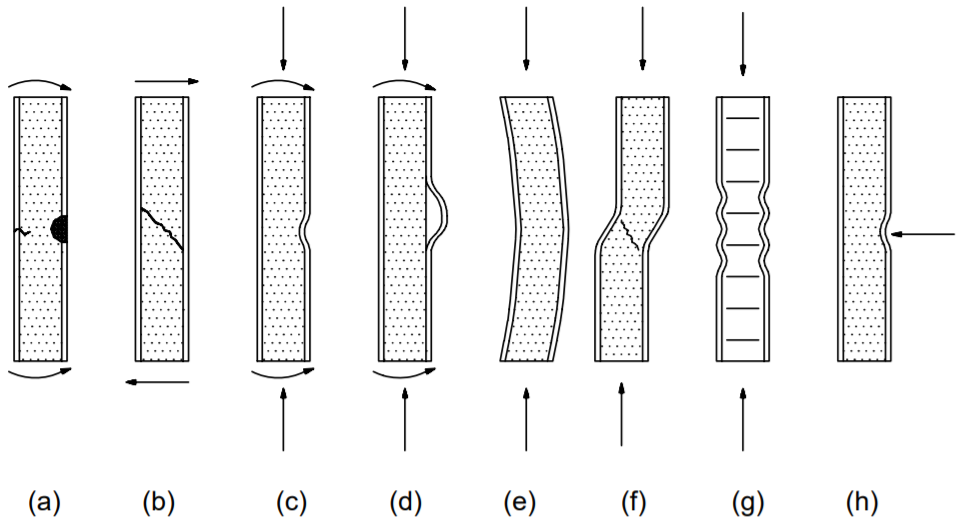
\includegraphics[width=0.65\textwidth]{04_Figures/Sandwich.png}
    \captionof{figure}{Versagensarten in Sandwichbalken.
                      (a) Fliessen/Bruch der Oberfläche,
                      (b) Schubbruch,
                      (c und d) Faltenbildung der Oberfläche,
                      (e) allgemeines Knicken,
                      (f) Scherfaltenbildung,
                      (g) Beulen an der Oberfläche und
                      (h) lokales Eindrücken.}
    \label{Sandwich}
  \end{center}

  Zu den Festigkeitsproblemen gehören;
  \begin{itemize}
    \item Fliessen der Deckschicht,
    \item Schubbruch der Kernschicht,
    \item Delamination und
    \item Ermüdung.
  \end{itemize}

  Zu den Stabilitätsproblemen gehören unteranderem;
  \begin{itemize}
    \item Knickung,
    \item Schubbeulung der Kernschicht (Shear Crimping) und
    \item Kurzwelliges Beulen der Deckschicht (Wrinkling).\\
  \end{itemize}

  Die auszulegenden Sandwichstrukturen werden gegenüber diesen Festigkeits und Stabilitätsproblemen ausgelegt.\\
  Um den Rechenaufwand und die Komplexität der Berechnungen zu verringern werden Annahmen und Vereinfachungen getroffen. Für die Auslegung von Sandwichstrukturen können folgende Annahmen getroffen werden \cite{klein}\cite{ETH};
  \begin{itemize}
    \item linear elastische und isentrope Materialverhalten,
    \item Eigenbiegesteifigkeiten der Deckschichten sind vernachlässigbar,
    \item Dehnsteifigkeit der Kernschicht ist vernachlässigbar und
    \item die Kernschicht lässt sich nicht zusammendrücken.\\
  \end{itemize}
  Aus den getroffenen Annahmen resultiert ein vereinfachter Spannungszustand, welcher besagt, dass die Deckschichten jeweils die Normalkräfte und die Kernschichten die Schubkräfte aufnehmen. (Sandwichmembrantheorie)

    \paragraph{Festigkeitsprobleme}\mbox{}\\
    Aus den getroffenen Annahmen und Vereinfachungen lassen sich die Formeln \ref{Spannung in Deckschicht} und \ref{Schubspannungen im Kern} herleiten. Mit der Formel \ref{Spannung in Deckschicht} lassen sich die Spannungen in den Deckschichten berechnen.

    \begin{equation}
      \label{Spannung in Deckschicht}
      \sigma_d = \frac{1}{t_d}\cdot \left ( \frac{n}{2} \pm \frac{m}{h}\right )
    \end{equation}

    Wobei $t_d$ für die Dicke der Deckschicht, $n$ für die Normalkraft pro Länge, $m$ für das Moment pro Länge und $h$ für die rechnerische Höhe der Platte stehen.

    Mit der Formel \ref{Schubspannungen im Kern} lassen sich die Schubspannungen in der Kernschicht berechnen und somit Aussagen über ihre Resistenz gegenüber dem Schubbruch machen.
    \begin{equation}
      \label{Schubspannungen im Kern}
      \tau_k = \frac{q}{t_k}
    \end{equation}

    Wobei $t_k$ für die Dicke der Kernschicht steht.

    Die Delamination der Deckschichten wird abgesichert, indem die Auswahl des Klebers, oder im Falle einer Laminierung die Wahl des Matrixwerkstoffes, so getroffen wird, dass dieser eine höhere Schubfestigkeit aufweist als das Material der jeweiligen Kernschicht.

    \paragraph{Stabilitätsprobleme}\mbox{}\\
    Die Stabilitätsprobleme der Sandwichstrukturen lassen sich in globale und lokale Instabilitäten einteilen. Zur globalen Instabilität gehört das Knicken, welches sich aus der Euler-Knickung des schubsteifen Balkens und dem Schubknicken zusammensetzt. Die kritische Belastung, bei welcher es zur Euler-Knickung kommt, lässt sich gemäss \emph{Klein} \cite{klein} mit der Formel \ref{Euler-Knicklast} berechnen.

    \begin{equation}
      \label{Euler-Knicklast}
      F_{kB}=\frac{\pi^2 \cdot E_d \cdot I}{l_k^{2}}
    \end{equation}

    Wobei sich das Widerstandsmoment $I$ vereinfacht gemäss der Formel \ref{ID} berechnen lässt. Hier wurde die Annahme getroffen, dass die Eigenbiegesteifigkeiten der Deckschichten vernachlässigbar sind. Diese Annahme kann gemäss \emph{Klein} ab einem Verhältnis von $t_d$ zu $t_k$ von 0.25, getroffen werden.
    \begin{equation}
      \label{ID}
      I= 2 \cdot b \cdot t_d \cdot \left( \frac{t_k}{2} + t_d \right )^{2}
      % B_y = 2\cdot b \cdot t_d\cdot \left ( \frac{t_k}{2}+t_d \right )^2
    \end{equation}

    Die kritische Schubknicklast lässt sich gemäss \emph{Klein} mit der Formel \ref{Schubknicklast} berechnen.
    \begin{equation}
      \label{Schubknicklast}
      F_{kS} = b \cdot t_k \cdot G_k
    \end{equation}

    Die totale kritische Knicklast \(F_k\) ergibt sich aus der Formel \ref{Knicklast}:
    \begin{equation}
      \label{Knicklast}
      F_{k, vorh.} \leq F_k=\frac{1}{\frac{1}{F_{kB}}+\frac{1}{F_{kS}}}
    \end{equation}

    Zu den lokalen Instabilitäten zählen das Schubbeulen und das Knittern der Deckschicht. Die kritischen Spannungen, bei welcher Schubbeulen auftritt, lässt sich aus den Formel \ref{Schubbeulen} berechnen. \cite{ETH}
    \begin{equation}
      \label{Schubbeulen}
      \sigma_k = G_k \cdot \frac{h}{2 \cdot t_d}
    \end{equation}

    Die kritischen Spannungen, bei welcher das Knittern der Deckschicht auftritt, lässt sich mit der Formel \ref{Knittern} berechnen. \cite{ETH}
    \begin{equation}
      \label{Knittern}
      \sigma_k = k_s\sqrt[3]{E_d \cdot E_k \cdot G_k}
    \end{equation}
    Wobei für Auslegungen \(k_s = 0.5\) gilt.

\newpage
  \subsubsection{Nieten}
    Für die Grobauslegung von Nietverbindungen wird angenommen, dass die angreifenden Schubkräfte gleichmässig auf die Anzahl Nieten in einer Verbindung verteilt werden. Anzahl und Typ der Nieten wird dabei so gewählt, dass die zulässige Scherkraft der Niete nicht überschritten wird. Laut Klein \cite{klein} gehört zum Tragfähigkeitsnachweis von Nietverbindungen für gewöhnlich ein Abscher- und Lochleibungsnachweis. Insofern sei für Nietverbindungen ein Nachweis auf Scherbruch (Formel \ref{Scherbruch}) und Lochleibung (Formel \ref{Lochleibung}) zu erbringen:
    \begin{multicols}{2}
      \begin{equation}
        \label{Scherbruch}
        F \leq F_{SB} = \frac{d_N^2 \cdot \pi}{4}\cdot \tau_B
      \end{equation}\break
      \begin{equation}
        \label{Lochleibung}
        F \leq F_{LF} = d_N \cdot t \cdot \sigma_{FL}
      \end{equation}
    \end{multicols}
    Wobei $d_N$ der Nietlochdurchmesser, $\tau_B$ die Scherfestigkeit, $t$ die Blechdicke und $\sigma_{FL}$ die Lochleibungs-Dehngrenze ist. Für dynamische Wechselfestigkeitswerte sei die Scherfestigkeit $\tau_B$ um den Faktor 2 bis 2.2 zu verringern.

    % \paragraph{Überlagerte Scher- und Zugbeanspruchung}
    % In der Praxis werden Nietverbindungen aus einer Kombination von Scher- und Zugbeanspruchung beansprucht. Der Nachweis der Tragfähigkeit der überlagerten Belastung wird durch die Ausweisung des Reservefaktors $R_f$ bewerkstelligt. Dazu werden gemäss den Formeln \ref{Rs} und \ref{Rz} der Schubreservefaktor $R_s$ und der Zugreservefaktor $R_z$ berechnet
    %
    % \begin{multicols}{2}
    %   \begin{equation}
    %     \label{Rs}
    %     R_s = \frac{F_s}{F_{SB}}
    %   \end{equation}\break
    %   \begin{equation}
    %     \label{Rz}
    %     R_z = \frac{F_z}{k \cdot F_{ZB}}
    %   \end{equation}
    % \end{multicols}
    %
    % Beim Verwenden von Vollnieten wird für $k$ der Wert 0.5, bei Blindnieten der Wert 0.2 verwendet.
    % Der Reservefaktor $R_f$ ergibt sich

  \subsubsection{Klebeverbindungen}
  Die Fähigkeit einer Klebeverbindungen Schubfluss zu übertragen, wird gemäss der Formel \ref{Kleben} beurteilt.
  \begin{equation}
    \label{Kleben}
    \tau_K = \frac{q}{b} \leq \frac{\tau_{KB}}{S}
  \end{equation}

  % Für dynamische Verbindungen werden folgende Abminderungsfaktoren verwendet. \cite{klein}
  % \begin{equation}
  %   \label{Zulässige Schubspannungen}
  %   \begin{split}
  %   wechselnd: & \: \tau_{KW} \approx \left (0.2 ... 0.4 \right ) \cdot \tau_{KB}\\
  %   schwellend: & \: \tau_{KSch} \approx 0.8 \cdot \tau_{KB}
  %   \end{split}
  % \end{equation}

\newpage

  \section{Lastenheft}
\label{Lastenheft}
In diesem Kapitel wird erklärt, wie das Lastenheft aufgebaut ist, wie die Lastfälle bestimmt und welche Annahmen dabei getroffen werden. Das Lastenheft ist auf der Seite \pageref{Lastenheft A} zu finden.\\

Damit die Erklärung des Lastenheftes und der gesamte folgende Auslegungsprozess an sich verständlicher wird, werden zuerst die verwendeten Begriffe definiert.

Als \emph{Modus} wird ein ``Zustand'' oder eine ``Position'' des Solar Butterflys verstanden. Modus \emph{A} beschreibt zum Beispiel den Solar Butterfly im ``Fahr-Modus''. In diesem Fall würde dies bedeuten, dass alle Panelen, Stützen und seitliche Raumelemente eingefahren sind.

Als \emph{Lastfall} wird eine Situation (z.B. Fahrt auf einer um 10° geneigten Strasse) oder eine Last (z.B. eine Personenlast) verstanden, welche in einem spezifischen Modus auftreten kann. Der Lastfall \emph{1.1} im Modus \emph{A} beschreibt zum Beispiel die vertikale Beschleunigung von 1.5 g welche durch das Überfahren einer Bremsschwelle auftreten kann. Der Lastfall \emph{1.1} im Modus \emph{C} beschreibt eine Personenlast.\\
Der Lastfall \emph{1.1} im Modus \emph{A} ist nicht notwendigerweise der Selbe, wie der Lastfall \emph{1.1} im Modus \emph{B} oder \emph{C}! Die klare Zuweisung der Lastfälle zu einem spezifischen Modus wurde vorgenommen, um die Anzahl der Lastfälle in den verschiedenen Modi gering zu halten und die daraus resultierenden Lastkombinationen pro Modus übersichtlicher zu gestalten. Dies führt mit sich, dass gewisse Lastfälle in mehreren Modi vorkommen und dass dadurch einige Lastfälle doppelt aufgeführt werden. So wird zum Beispiel der Lastfall \emph{Neigung längs positiv} im Modus \emph{B} und \emph{C} aufgeführt, da die Situation des geneigten Bodens im parkierten Zustand in beiden Modi auftreten kann. Alle Lastfälle, welche in diesen Modi nicht auftreten, können jedoch weggelassen werden, wodurch - wie bereits erwähnt - das Lastenheft übersichtlicher gestaltet werden kann.

Zur Beschreibung eines Lastfalles gehört eine Bewertung des dazugehörenden \emph{Risikos}. Ein \emph{Risiko} setzt sich zusammen aus der Ungenauigkeit der Voraussage einer Belastung und einer Abschätzung der ``Ernsthaftigkeit'' der Auswirkungen, sollte die Ungenauigkeit eintreten. Eine \emph{Ungenauigkeit} von 0.5 bedeutet, dass von einer potenziellen Abweichung der Belastung von $\pm\: 50\%$ ausgegangen wird. Für die Werte der \emph{Auswirkungen} wird kein klarer Massstab definiert. Sie nehmen Werte zwischen 0 und 100 an und beurteilen die Auswirkungen beim Eintreten der Ungenauigkeit. Das Produkt aus der Ungenauigkeit und der Auswirkung ergibt den Wert des Risikos.\\
Ein hoher Risikowert bedeutet nicht, dass die betreffende Last ein grosses Risiko für den Solar Butterfly darstellt, sondern, dass die Abschätzung der Last unsicher ist. Das soeben erläuterte Risiko ist also ein Mass für die Gefahr, sowie auch für das Potenzial, welches in der Abschätzung der Last steckt. Ein Risikowert von 0 bedeutet ausgeschrieben, dass die Last mit grosser Sicherheit so auftreten wird, wie diese im Lastenheft beschrieben ist oder, dass falls eine Abweichung der Last auftreten sollte, die Auswirkungen äusserst gering sind. Ein hoher Risikowert bedeutet wiederum, dass man sich nicht sicher ist, ob die Last wie beschrieben auftreten wird oder dass falls eine Abweichung auftreten würde, diese grosse Auswirkungen haben wird. Die Last kann zu tief (daher die Gefahr), oder aber auch zu hoch (daher das Potential) gewählt worden sein. Lasten mit hohen Risikowerten sollen bei einer eventuellen Überarbeitung des Lastenheftes erhöhte Beachtung geschenkt werden.

Als \emph{Lastkombination} wird eine Kombination von verschiedenen Lastfällen verstanden. Eine Lastkombination bezieht sich jeweils auf einen Modus. Die Lastkombination \emph{A.3.1.2} setzt sich zum Beispiel zusammen aus dem Modus \emph{A} und den Lastfällen \emph{1.3 Longitudinale Beschleunigung - Negativ}, \emph{2.1 Wind von links} und \emph{3.2 Neigung längs negativ} aus dem Modus \emph{A}. Die zweite Zahl im Namen der Lastfälle tritt jeweils im Namen der Lastkombination auf.

\subsection{Missbrauchslastfälle}
Als Missbrauchslastfälle werden die im Lastenheft nicht aufgeführte Situationen oder Ereignisse verstanden, an welchen der Solar Butterfly Schaden nehmen könnte. Beispiele von Missbrauchslastfällen sind kleinere Unfälle, stolpernde Personen und unsachgemässe Bedienung. Der Solar Butterfly wird gegenüber den Lasten im Lastenheft ausgelegt, die Missbrauchslastfälle werden bei der Auslegung und Konstruktion der einzelnen Komponenten jedoch berücksichtigt.

\subsection{Dynamik}
Die Dynamik der Lastfälle wird in der Grobauslegung nicht im Detail betrachtet. Der Solar Butterfly wird jeweils für den Maximalwert (Amplitude) eines Lastfalles statisch ausgelegt. Die Dynamik der Lastfälle und die daraus resultierende potenzielle Ermüdung der Materialien, wird in der Grobauslegung mit entsprechend gewählten Design-Allowables und gutem Design abgedeckt.

\subsection{Modus A: Fahren}
Der Modus \emph{A} beschreibt den Solar Butterfly im ``Fahr-Modus'' und ist in der Abbildung \ref{Modus A} dargestellt. Konkret bedeutet dieser Modus, dass alle Panelen und seitliche Raumelemente eingefahren und über die Verschlüsse fest mit dem Rest des Aufbaus verbunden sind. Ebenfalls sind alle Stützen eingefahren. Im Fahr-Modus befinden sich keine Personen im Solar Butterfly und das Mobiliar ist an den dafür vorgesehenen Stellen verstaut. Weiter herrscht in allen Lastkombinationen die Erdbeschleunigung von 1 g. Der Lastfall von 1 g wird nicht spezifisch aufgeführt.

\begin{center}
  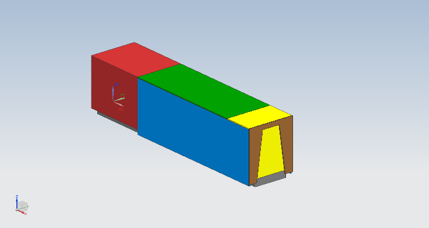
\includegraphics[width=0.5\textwidth]{04_Figures/A.png}
  \captionof{figure}{Modus A}
  \label{Modus A}
\end{center}

  \paragraph{Beschleunigungen während der Fahrt}
  \begin{description}
    \item \textbf{1.1 Vertikale Beschleunigung}\\
    Zusätzlich zur vertikalen Beschleunigung durch die Erdanziehung können durch das Überfahren von Schlaglöchern und Bremsschwellen vertikale Beschleunigungen entstehen.\\
    In einem ersten Ansatz, die vom Solar Butterfly erfahrene Beschleunigung beim Überfahren einer Bremsschwelle zu bestimmen, wird der Solar Butterfly als ein Einmassenschwinger-System modelliert und die Beschleunigung beim Überfahren einer Sinusförmigen Bremsschwelle numerisch ermittelt.\\
    Der Rechnungsweg wird im Anhang \ref{Vertikale Beschleunigung} ausführlich erläutert und die Exceltabelle, mit welcher die Berechnung durchgeführt wurde, ist im elektronischen Anhang \ref{e:Lastenheft} zu finden.

    Das \emph{Ein-Massen-Schwinger}-Modell wurde mit einer Masse von 3000 kg, einer mittleren Federkonstante, bestimmt aus den Datenblättern des Herstellers (elektronischer Anhang \ref{e:Federkonstante}), von 353'000 N/m und mit einer Dämpfungskonstante von 10000 Ns/m (5000 Ns/m pro Achse) modelliert. Als Anhaltswert für die Wahl der Dämpfungskonstante wurde die Dämpfungskonstante von 5000 Ns/m pro Achse eines 2500 kg schweren SUV's gewählt \cite{Beschl.2}. Beim Überfahren einer Bremsschwelle von 0.9 m Länge und 0.1 m Höhe, mit einer Geschwindigkeit von 40 km/h, resultiert eine maximale Beschleunigung von rund 1.7 g.\\
    Zu diesem Ergebnis muss gesagt werden, dass davon ausgegangen werden kann, dass die erhaltene Beschleunigung zu hoch liegt. So wurde zum Beispiel die Effekte der Reifen und die rotatorische Trägheit des Solar Butterflys nicht berücksichtigt, was Abminderungen der berechneten Beschleunigung zur Folge hätten. Dennoch wird der erhaltene Wert als guten Vergleichswert und Anhaltspunkt für weitere Abklärungen gehalten.

    Um die zu wählende Beschleunigung breiter abstützen zu können, wurden andere Arbeiten zum Thema herbeigezogen. \emph{Janczur} \cite{Beschl.1} zeigt, dass beim Überfahren einer Bremsschwelle von 0.36 m Länge und einer Höhe von 0.05 m, mit einer Geschwindigkeit von 40 km/h, in der Fahrzeugmitte eines Personenwagens, Beschleunigungen von 0.71 g herrschen. Direkt über der Fahrzeugachse treten Beschleunigungen von bis zu 1.5 g auf.\\
    \emph{García-Pozuelo} et al. \cite{Beschl.2} massen in der Fahrzeugmitte eines Personenwagens Beschleunigungen von 0.73 g beim Überfahrein einer Bremsschwelle von 0.9 m Länge und 0.1 m Höhe. Dies bei einer Geschwindigkeit von 50 km/h.\\
    \emph{Haniszewski} et al. \cite{Beschl.3} massen Beschleunigungen, welche eine Person auf der Rückfahrbank eines Personenwagens, während dem Überfahren einer Bremsschwelle erfährt. Sie massen Beschleunigungen von bis zu 1 g. Direkt über der Fahrzeugachse wurden Beschleunigungen von 1.3 g gemessen. Dies bei einer Geschwindigkeit von 30 km/h und einer Bremsschwelle von 0.5 m Länge und 0.05 m Höhe.\\
    \emph{Pidl} \cite{Beschl.4} zeigt, dass Transportware in einem Sattelschlepper Beschleunigungen von $\pm$ 1 g erfahren. Ob diese maximal gemessene Beschleunigung beim Überfahren einer Bremsschwelle erreicht wurde, ist nicht ersichtlich.

    Da der Achsenabstand des Solar Butterflys, im Vergleich zu den Personenwagen aus der Literatur, relativ klein ist, werden die in der Fahrzeugmitte gemessenen Beschleunigungen der Personenwagen nicht als repräsentative Näherungswerte für die Beschleunigung des Solar Butterflys verwendet. Es wird davon ausgegangen, dass die Beschleunigungen, welcher ein Personenwagen direkt über der Achse beim Überfahren einer Bremsschwelle erfährt, vergleichbar mit jenen sind, welche der Solar Butterfly erfahren wird. Diese Annahme wird getroffen, da die Achsen des Solar Butterflys nahe beisammen liegen und eher den letzteren Fall beschreiben.\\
    Aufgrund der getroffenen Annahmen wird die Beschleunigung von 1.5 g als erste Abschätzung festgelegt. Hinsichtlich der grossen Unsicherheit der Annahmen wird die \emph{Ungenauigkeit} auf 0.4 geschätzt. Die \emph{Auswirkung} werden dabei mit einem Wert von 50 festgelegt was den hohen Risikowert von 20 ergibt.

    \item \textbf{1.2 Longitudinale Beschleunigung - Positiv (Erhöhen der Geschwindigkeit)}\\
    Longitudinale positive Beschleunigungen in Fahrtrichtung entstehen durch eine Erhöhung der Fahrgeschwindigkeit durch das Zugfahrzeug. Das \emph{Institut für Unfallanalysen Hamburg} \cite{Verz.3} benützt die Beschleunigung von Personenwagen von maximal 0.3 g und von Lastkraftwagen von 0.1 g, als Anhaltswerte.

    Für das Lastenheft wird die Beschleunigung von 0.2 g gewählt. Sie wird höher als der Anhaltswert des Institut für Unfallanalysen Hamburg für Lastkraftwagen von 0.1 g gewählt, da das geplante Zugfahrzeug ein elektrisches ist, und dadurch höhere mögliche Beschleunigungen erwartet werden können.\\
    Die \emph{Ungenauigkeit} wird mit 0.2 als gering eingestuft. Ebenfalls wird die \emph{Auswirkung} mit 20 als niedrig bewertet.

    \item \textbf{1.3 Longitudinale Beschleunigung - Negativ (Bremsen)}\\
    Longitudinale Verzögerungen entstehen durch Abminderung der Fahrgeschwindigkeit. Die extremste graduelle Verzögerung entsteht dabei durch eine Notbremsung.\\
    \emph{Kudarauskas} \cite{Verz.1} zeigt bei seiner Analyse der Notbremsungen von Personenwagen, dass die maximalen Verzögerungen bei rund 0.9 g liegen. Das \emph{Institut für Unfallanalysen Hamburg} \cite{Verz.2} zeiht bei Gutachten die Vollverzögerung von 0.8 g für Personenwagen und 0.7 g für Lastkraftwagen als Standardwerte herbei.

    Für die longitudinale Beschleunigung durch Bremsungen wird sich am Institut für Unfallanalysen Hamburg orientiert und ein Wert von 0.7 g gewählt. Dies, da davon ausgegangen wird, dass die maximalen Verzögerungen von \emph{Kudarauskas} von 0.9 g mit dem Solar Butterfly nicht erreicht werden können. Weiter wird angenommen, dass das Verhalten eines Lastkraftwagens während einer Vollverzögerung die Situation des Solar Butterflys ähnlicher beschreibt als jenes des Personenwagens.
    Die longitudinale Beschleunigung wird mit einer \emph{Ungenauigkeit} von 0.2 und einer \emph{Auswirkung} von 30 bewertet.

    \item \textbf{1.4 Laterale Beschleunigung}\\
    Laterale Beschleunigungen entstehen vor allem beim Kurvenfahren und sind abhängig von der Geschwindigkeit, mit welcher die Kurve durchfahren wird und des Kurvenradius.\\
    \emph{Hugemann} et al. \cite{Kurv.1} massen in einem Personenwagen auf einer Landstrasse laterale Beschleunigungen von 0.6 g. \emph{Xu} et al. \cite{Kurv.2} zeigen, dass die Mehrheit der gemessenen Beschleunigungen in einem Personenwagen durch Kurvenfahrten in bergigem Gebiet über 0.5 g und die maximalen über 0.8 g liegen.

    Da davon ausgegangen wird, dass mit dem Solar Butterfly Kurven tendenziell vorsichtiger, und somit eher langsamer durchfahren werden als mit einem Personenwagen, wird die laterale Beschleunigung von 0.8 g als ein passenden Anhaltswert erachtet. Es wird erwartet, dass die nach \emph{Xu} et al. höher als 0.8 g liegende Beschleunigungen nicht erreicht werden. Die \emph{Ungenauigkeit} wird mit 0.1 als gering bewertet. Die \emph{Auswirkung} wird auf 70 geschätzt.

    \item \textbf{1.5 Rotatorische Beschleunigung}\\
    Rotatorische Beschleunigungen können durch eine in Querrichtung unebene Strassen verursacht werden. Beim Überfahren einer solchen Strasse neigt sich der Solar Butterfly abwechslungsweise nach links und rechts, wodurch rotatorische Beschleunigungen auftreten. Um diese Beschleunigungen abschätzen zu können wird die folgende Berechnung durchgeführt:

    Die folgende Gleichung beschreibt den Neigungswinkel $\varphi$ des Solar Butterflys in Abhängigkeit der Zeit $t$:
    \begin{equation}
      \varphi(t) = \varphi \cdot \sin \left(\omega t \right)
    \end{equation}

    wobei $\varphi$ für die maximale Neigung steht und die Kreisfrequenz $\omega$ sich wie folgt berechnen lässt:
    \begin{equation}
      \omega = \frac{2\cdot \pi}{T}
    \end{equation}
    Wobei $T$ für die Dauer einer Schwingung (Neigung von rechts nach links und wieder zurück) steht.\\
    Die Winkelbeschleunigung $\alpha$ ergibt sich aus der zweiten Ableitung von $\varphi(t)$ und lässt sich wie folgt berechnen:
    \begin{equation}
      \alpha(t) = \ddot \varphi(t) = -\Delta\varphi\:\omega^2 \cdot \sin \left(\omega t \right)
    \end{equation}

    Mit einer Schwingdauer von einer Sekunde und einer maximalen Neigung $\varphi$ von 6.5° (vgl. Abbildung \ref{1.5 Skizze}), welche sich aus einem Höhenunterschied des Rades von 200 mm und dem Radstand des Solar Butterflys von 1770 mm ergibt, resultiert eine maximale Winkelbeschleunigung von $4.4 \; \frac{rad}{s^2}$.\\
    Da die realen Bedingungen einer solchen Situation nur schwer abgeschätzt werden können, wird die \emph{Ungenauigkeit} mit 0.3 hoch angesetzt. Ebenfalls können die Auswirkungen einer solchen Beschleunigung nur schwer beurteilt werden, weshalb die \emph{Auswirkung} auf 60 gesetzt wird.

    \begin{center}
      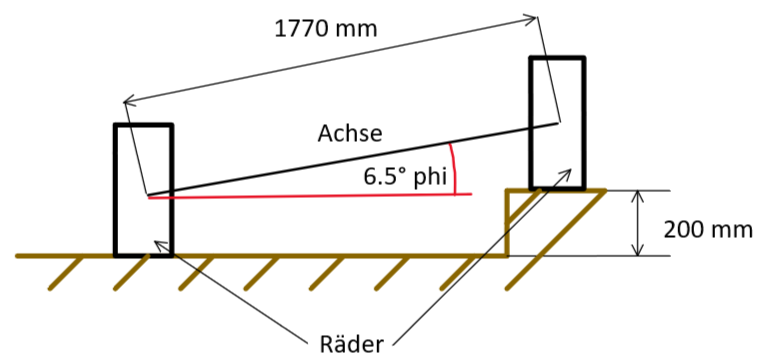
\includegraphics[width=0.6\textwidth]{04_Figures/1.5 Skizze.png}
      \captionof{figure}{Skizze zur Beschreibung des Neigungswinkel $\varphi$}
      \label{1.5 Skizze}
    \end{center}

  \end{description}

  \paragraph{Windlasten}\mbox{}\\
  \emph{Sesar} et. al \cite{Wind.1} zeigen, dass laterale Windgeschwindigkeiten von 108 $\frac{km}{h}$ für fahrende Fahrzeuge auf trockener Strasse kritische seien.\\
  Die Blog-Seite \emph{rvblogger.com} \cite{Wind.2} empfiehlt bei Windgeschwindigkeiten von mehr als 80 $\frac{km}{h}$ mit einem Wohnwagen nicht mehr zu Fahren. Windgeschwindigkeiten von 95 $\frac{km}{h}$ seien laut \emph{rvblogger.com} genug, um Wohnmobile umzustossen.\\
  Bei Windgeschwindigkeiten von mehr als 155 km/h können laut \emph{Beasley} \cite{Wind.3} Lastwagen mit hohem Profil, Anhänger und Busse umkippen. Die berichteten minimale Überschlagswindgeschwindigkeiten sind 105 $\frac{km}{h}$ für ein 9 Meter langen Wohnwagen und 160 $\frac{km}{h}$ für ein 5 Meter langes Wohnmobil (Klasse B).

  Für eine erste Abschätzung der zugelassenen Windgeschwindigkeit bei der Fahrt des Solar Butterfly wird sich an der Blog-Seite \emph{rvblogger.com} orientiert und die Geschwindigkeit von 80 $\frac{km}{h}$ als Limitte festgelegt. Für die Berechnung der durch den Wind entstehenden Belastung, wird der Solar Butterfly vereinfacht als normal angeströmtes Rechteck betrachtet. Für die Berechnung des Winddruckes wird die erhöhte Geschwindigkeit von 102.2 $\frac{km}{h}$ (Beaufort 10) verwendet, um Windböen und eventuelle Ungenauigkeiten in der Messung oder Abschätzung der Windgeschwindigkeiten abzudecken. Der Winddruck wird gemäss Formel \ref{Winddruck} berechnet.

  \begin{equation}
    \label{Winddruck}
    P_W = c_p \: \frac{\rho}{2}\: v^2
  \end{equation}

  Wobei für die Dichte von Luft $\rho$ ein Wert von $1.2 \frac{kg}{m^3}$ und für den Strömungswiderstandskoeffizient eines Rechteckes $c_{p,Rechteck}$ ein Wert von $1.1$ gewählt wird. Bei einer Windgeschwindigkeit von 102.2 $\frac{km}{h}$ ergibt sich gemäss der Gleichung \ref{Winddruck} ein Winddruck von $532 \; Pa$.

  Da es sich hierbei um eine grobe Idealisierung handelt und zum Beispiel lokale Geschwindigkeitserhöhungen oder Turbulenzen vernachlässigt werden, wird die \emph{Ungenauigkeit} auf 0.4 gesetzt. Die \emph{Auswirkung} wird jedoch eher tief, mit dem Wert 10 bewertet.

  Im Lastenheft werden zwei Windlasten mit dem oben berechneten Winddruck aufgeführt. Die beiden Windlasten unterscheiden sich dabei in ihrer Anströmung. (Anströmung von Links und Rechts)

  % \begin{description}
  %   \item \textbf{2.1 Wind von links}\\ Der Winddruck von $532  \; Pa$ wirkt auf die, in Fahrtrichtung gesehen, linke Seite des Solar Butterfly.
  %   \item \textbf{2.2 Wind von rechts}\\ Der Winddruck von $532 \; Pa$ wirkt auf die, in Fahrtrichtung gesehen, rechte Seite des Solar Butterfly.
  % \end{description}

  \paragraph{Neigung}\mbox{}\\
  Mittels einer Absprache mit \emph{Palmer} wurde eine zulässige Strassenneigung für den Solar Butterfly von 10° (17.5\%) definiert (vgl. Pflichtenheft 10.0.3 Max. Neigung Fahrt). Die Strasse auf den Furkapass hat zum Vergleich eine maximale Neigung von 6.3° (11\%). Die verschiedenen Lastfälle der Neigung treten nicht gleichzeitig ein. Implementiert werden die Fälle in einer FEM-Berechnung, indem die Richtung, in welcher die Erdbeschleunigung wirkt, verändert wird. Im Lastenheft werden vier verschiedene Neigungslasten definiert, welche sich jeweils in ihrer Richtung der Neigung unterscheiden.\\
  Die \emph{Ungenauigkeit} und die \emph{Auswirkung} werden tief mit den Werten 0.1 und 10 bewertet.



  % \begin{description}
  %   \item \textbf{3.1 Neigung längs positiv} +10° Neigung des Untergrundes in Fahrtrichtung.
  %   \item \textbf{3.2 Neigung längs negativ} -10° Neigung des Untergrundes in Fahrtrichtung.
  %   \item \textbf{3.3 Neigung quer positiv} +10° Neigung des Untergrundes noraml zur Fahrtrichtung. Ansteig befindet sich in Fahrtrichtung rechts.
  %   \item \textbf{3.4 Neigung quer negativ} -10° Neigung des Untergrundes noraml zur Fahrtrichtung. Ansteig befindet sich in Fahrtrichtung links.
  % \end{description}

  % \paragraph{Mobiliar}\mbox{}\\
  % Gemäss der Anforderungsliste werden sich bis zu 50 kg Mobiliar im Solar Butterfly befinden. Während der Fahrt (Modus A) befindet sich das Mobiliar an der Seitenwand im inneren Seitenmodul.
  %
  % \emph{Ungenauigkeit} 0.4, da grosse ungewissheit bei der Befestigung des Mobiliars. Art der Einleitung ist unbekannt.
  % \emph{Auswirkung} 20, ebenfalls nicht zu vernachlässigen da je nach Art der Befestigung die Konstruktion angepasst werden muss.
  % \begin{description}
  %   \item \textbf{4.1 Mobiliar}\\
  %   !!!!! Wie wird das im FEM gemacht? !!!!!
  % \end{description}

  %=============================================================================
  %                                 Modus B
  %=============================================================================
\subsection{Modus B: Ausfahren}
Die Modi \emph{B1}, \emph{B2} und \emph{B3} beschreiben den Solar Butterfly während dem Ausfahrvorgang der seitlichen Raumelemente. Im Modus \emph{B1} sind die Stützen am Chassis unten und alle seitlichen Raumelemente und Panelen sind eingefahren. Dieser Modus stellt den Solar Butterfly im ``Abgestellten'' Zustand dar. Bei extremen Umwelteinflüssen wie Schneefall oder starkem Wind, stellt der Modus \emph{B1} den geschütztesten Zustand dar und muss somit diesen extremen Umwelteinflüssen standhalten können.
Im Modus \emph{B2} ist, zusätzlich zu den Stützen am Chassis, das grosse seitliche Raumelement (In der Abbildung \ref{Modus B2} orange dargestellt) ausgefahren. Standardmässig werden beide seitlichen Raumelemente zur selben Zeit ausgefahren. Sollte dies aufgrund von technischen Problemen nicht möglich sein und die Raumelemente müssen ``von Hand'' einzeln ein- oder ausgefahren werden, wird der Modus \emph{B2} eingenommen. Im Modus \emph{B3} ist zusätzlich das zweite seitliche Raumelement ausgefahren.\\
Auch in diesen drei Modi herrscht die Erdbeschleunigung von 1 g, welche wiederum nicht als Lastfall aufgeführt wird. Während dem Ausfahrvorgang befinden sich keine Personen im Fahrzeug und das Mobiliar befindet sich an der dafür vorgesehenen stellen, wie dies im Modus \emph{A} zuvor bereits der Fall war.

\begin{figure}[!ht]
  \centering
    \begin{subfigure}{.333\textwidth}
      \centering
      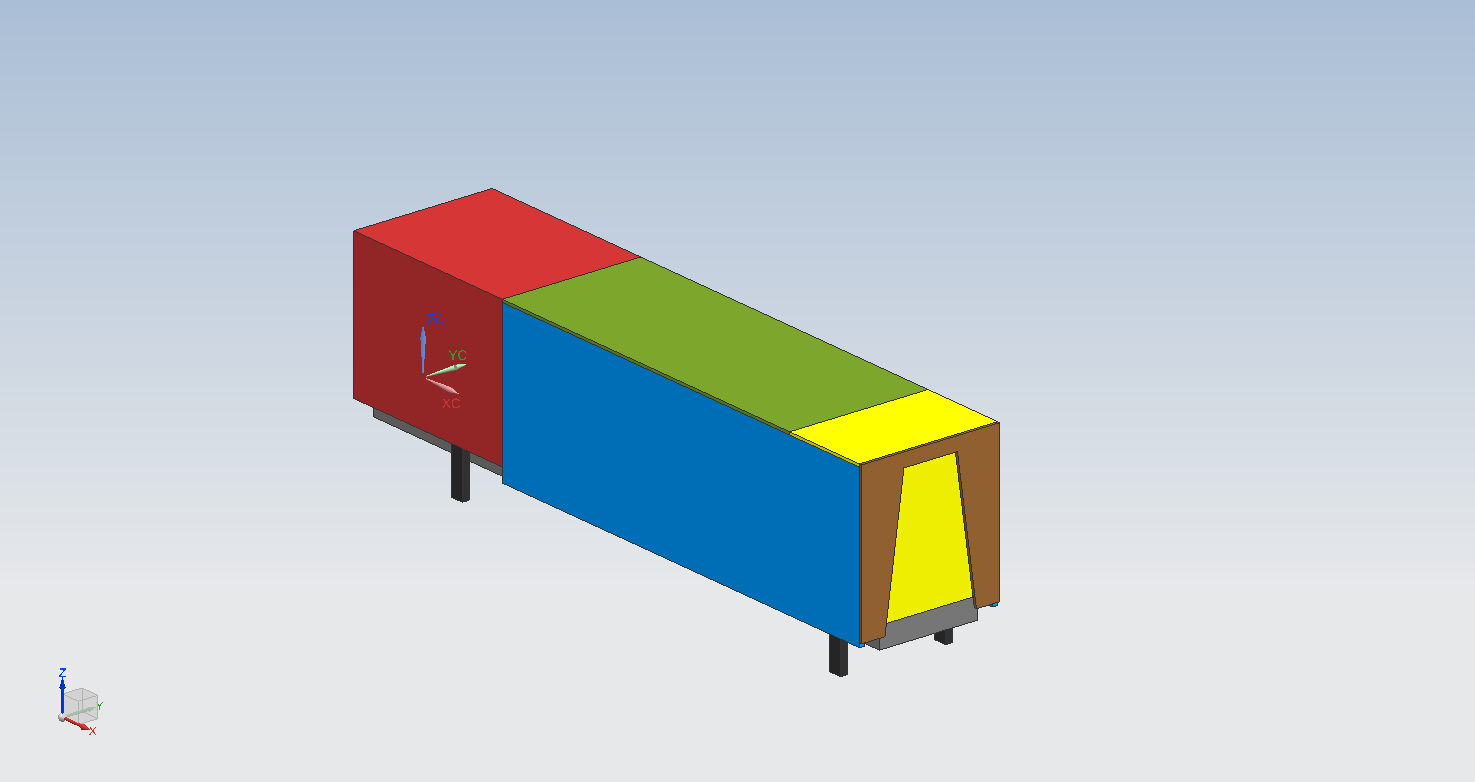
\includegraphics[width=.98\linewidth]{04_figures/B1.png}
      \caption{Modus B1}
      \label{Modus B1}
    \end{subfigure}%
    \begin{subfigure}{.333\textwidth}
      \centering
      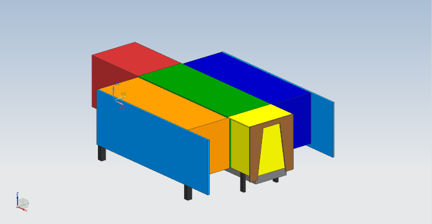
\includegraphics[width=.98\linewidth]{04_figures/B2.png}
      \caption{Modus B2}
      \label{Modus B2}
    \end{subfigure}%
    \begin{subfigure}{.333\textwidth}
      \centering
      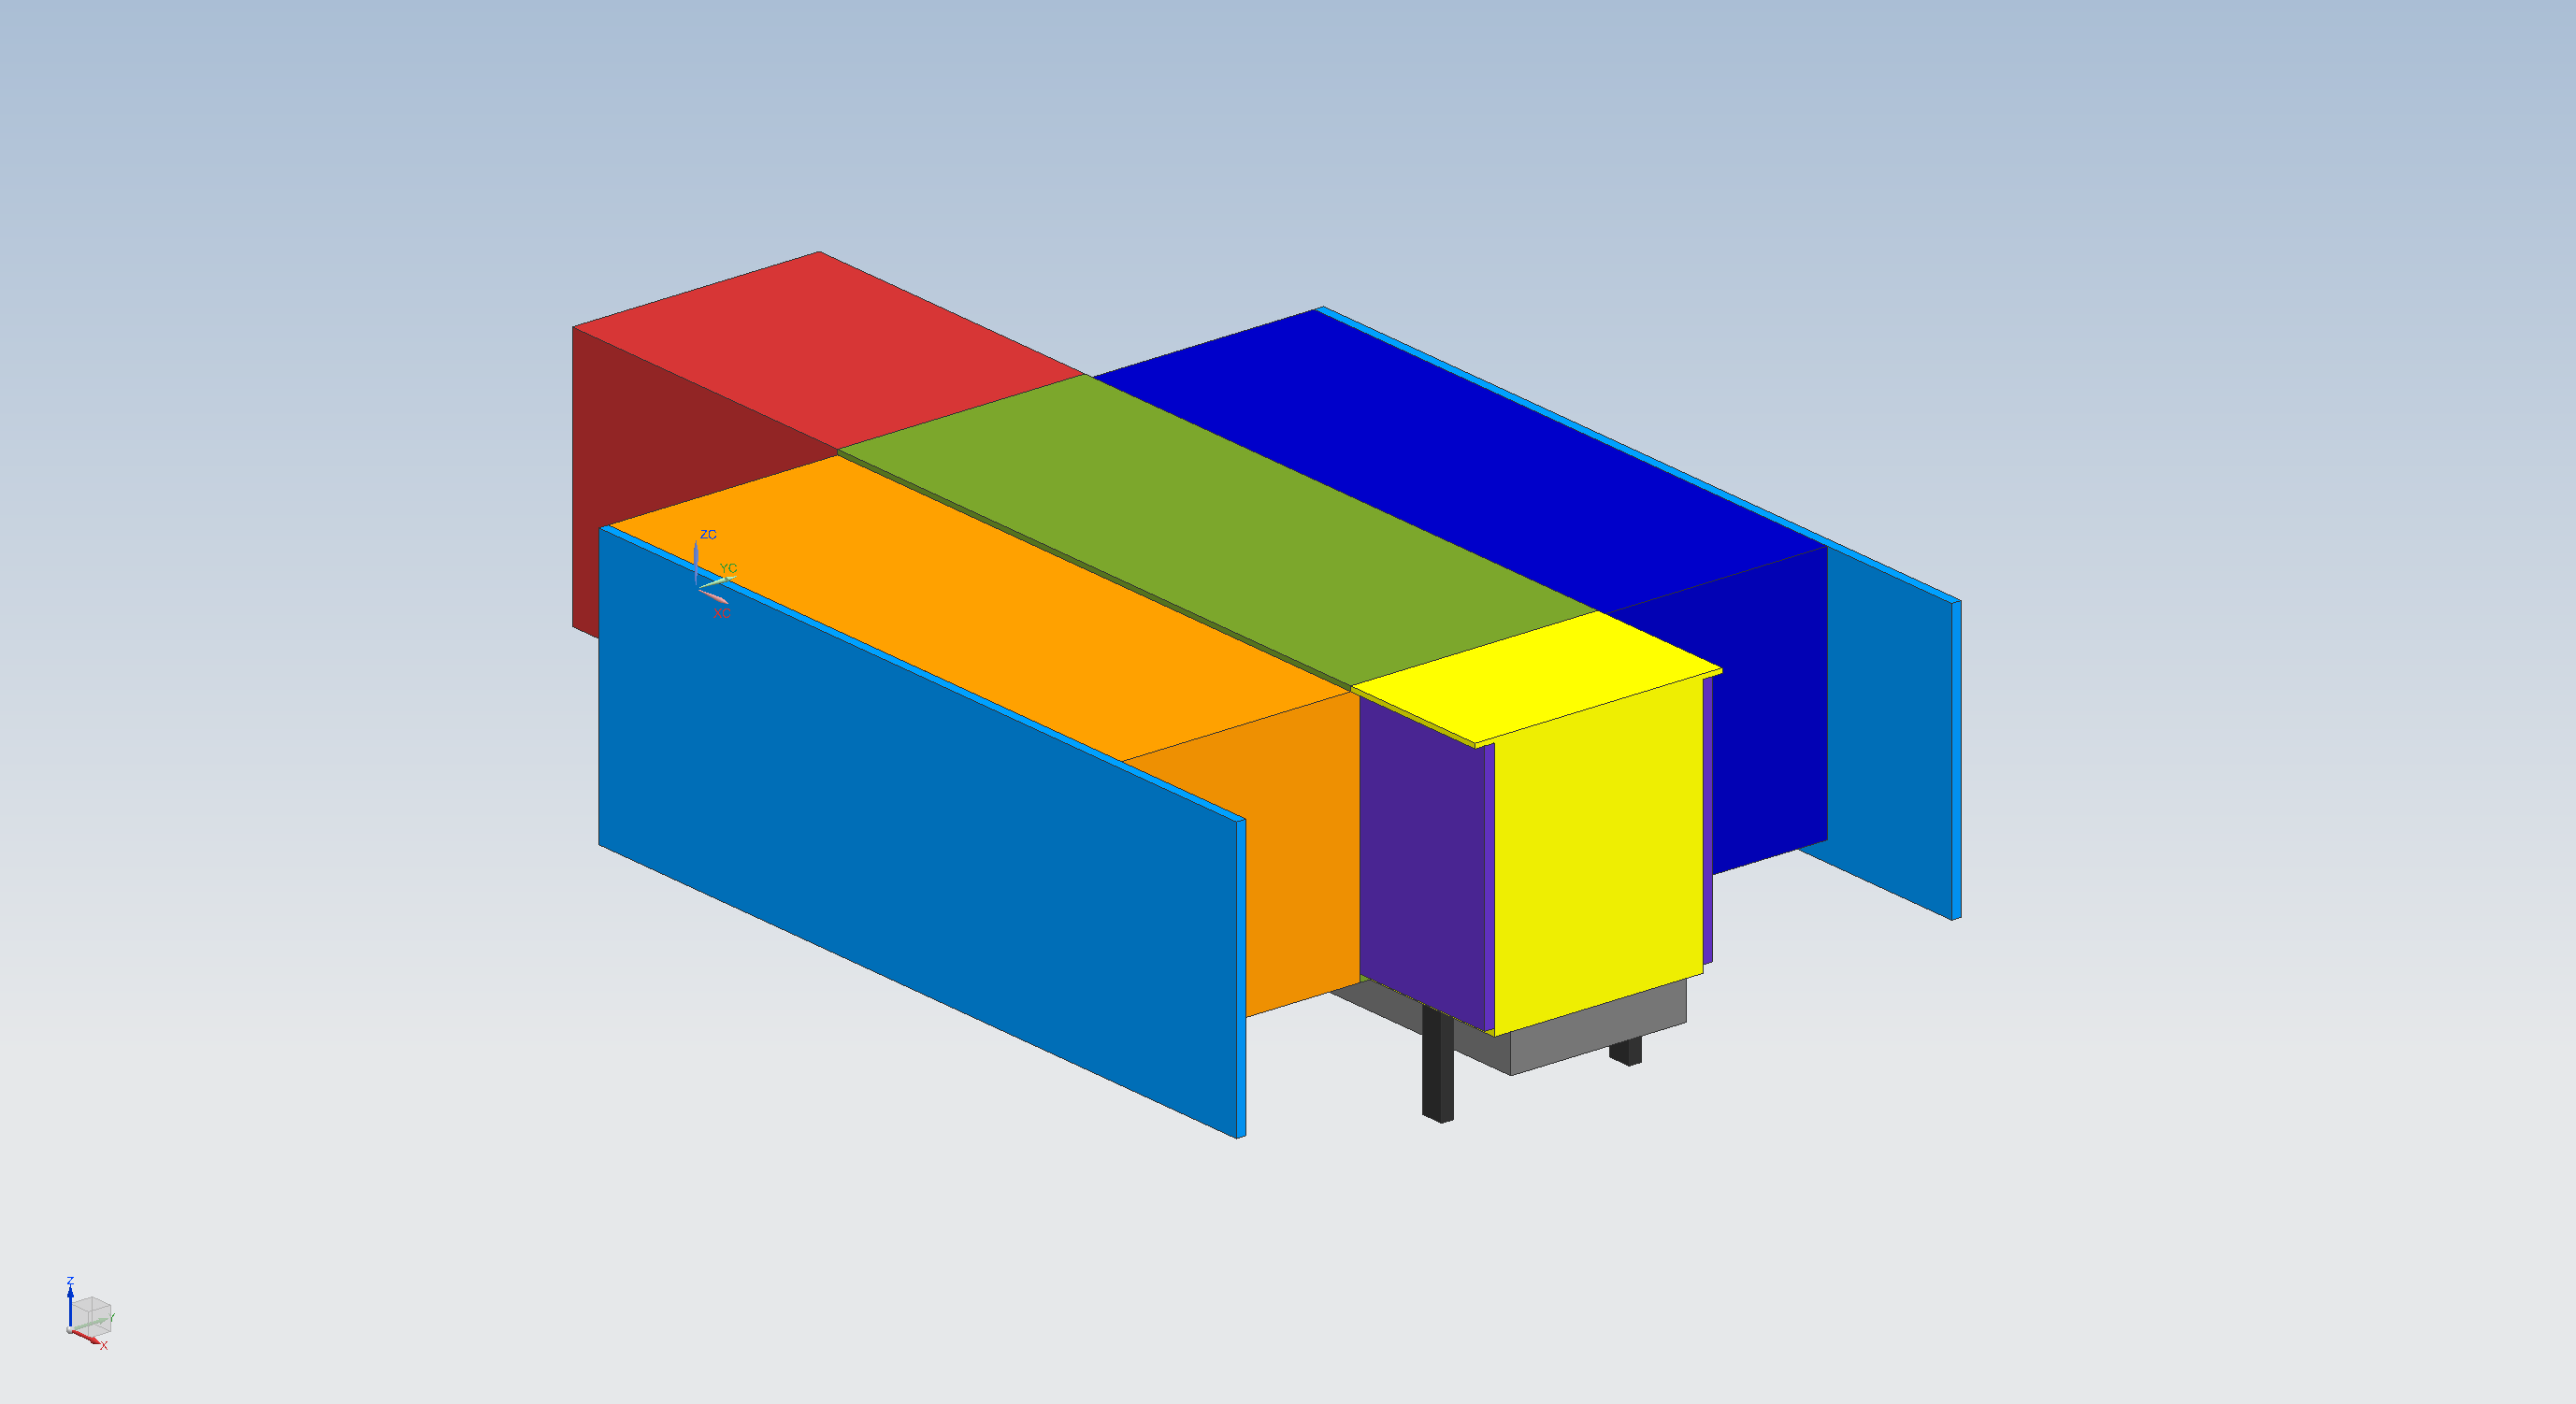
\includegraphics[width=.98\linewidth]{04_figures/B3.png}
      \caption{Modus B3}
      \label{Modus B3}
    \end{subfigure}
  \caption{Modi beim Ausfahren}
\label{Modi beim Ausfahren}
\end{figure}

\paragraph{Windlasten}\mbox{}\\
Als Windlasten im Modus \emph{B} werden vier Lastfälle definiert, wobei zwei davon ``extreme'' Windlasten darstellen. Den beiden extremen Windlasten, welche sich aus einer Windgeschwindigkeit von 125 km/h (Beaufort 12: Orkan) ergeben, müssen nur im Modus \emph{B1} standgehalten werden. Die beiden gemässigteren Windlasten entstehen aus Windgeschwindigkeiten von rund 70 km/h (Beaufort 8: Stürmischer Wind).\\
Die \emph{Ungenauigkeit} der extremen Lastfälle wird auf 0.4 und die \emph{Auswirkungen} auf 40 geschätzt. Für die beiden anderen Windlasten werden die Werte 0.4 und 20 verwendet.
% Windlast von Panelen übernommen. Verweis auf \emph{Bauholzer}
% \begin{description}
%   \item \textbf{1.1 Wind extrem links}\\
%   \item \textbf{1.2 Wind extrem rechts}\\
%   Winddruck bei 120 km/h (Orkan, Beaufort 12)?\\
%   Eher unsicher, kann viel höher liegen. daher nur erste annahme\\
%   Ungenauigkeit 0.4, Auswirkungen 40
%
%   \item \textbf{1.3 Wind von links}\\ Der Winddruck von $486 \; Pa$ wirkt auf die, in Fahrtrichtung gesehen, linke Seite des Solar Butterfly.
%   \item \textbf{1.4 Wind von rechts}\\ Der Winddruck von $486 \; Pa$ wirkt auf die, in Fahrtrichtung gesehen, rechte Seite des Solar Butterfly.
%   Winddruck bei 120 km/h (Orkan, Beaufort 10)?\\
%   Eher unsicher, kann viel höher liegen. daher nur erste annahme\\
%   Ungenauigkeit 0.4, Auswirkungen 20
% \end{description}

\paragraph{Neigung}\mbox{}\\
Mit Palmer wurde abgesprochen, dass der Boden, auf welchem der Solar Butterfly parkiert wird, die Neigung von 5° (8.8\%) nicht überschreiten darf (vgl. Pflichtenheft 10.0.4 und 10.0.5 Max. Neigung im Stand). Die Implementierung und Risikobewertung der Lastfälle werden analog zu den Neigungsfällen im Modus \emph{A} durchgeführt.

% \begin{description}
%   \item \textbf{2.1 Neigung längs positiv} +5° Neigung des Untergrundes in Fahrtrichtung.
%   \item \textbf{2.2 Neigung längs negativ} -5° Neigung des Untergrundes in Fahrtrichtung.
%   \item \textbf{2.3 Neigung quer positiv} +5° Neigung des Untergrundes noraml zur Fahrtrichtung. Ansteig befindet sich in Fahrtrichtung rechts.
%   \item \textbf{2.4 Neigung quer negativ} -5° Neigung des Untergrundes noraml zur Fahrtrichtung. Ansteig befindet sich in Fahrtrichtung links.
% \end{description}

% \paragraph{Mobiliar}\mbox{}\\
% Der Lastfall des Mobiliars wird analog zum Lastfall \emph{4.1 Mobiliar} im Modus \emph{A} implementiert und wird hier nur der Vollständigkeit halber aufgeführt.
% \begin{description}
%   \item \textbf{3.1 Mobiliar}\mbox{}\\
%   Bla Bla. Text von oben kopieren.
% \end{description}

%=============================================================================
%                                 Modus C
%=============================================================================
\subsection{Modus C: Ausgefahren}
Der Modus \emph{C} beschreibt den Solar Butterfly im parkierten und voll ausgefahrenen Zustand. Alle Panelen, seitlichen Raumelemente und Stützen sind ausgefahren. Personen und das Mobiliar können frei im Solar Butterfly verteilt sein.\\

\begin{center}
  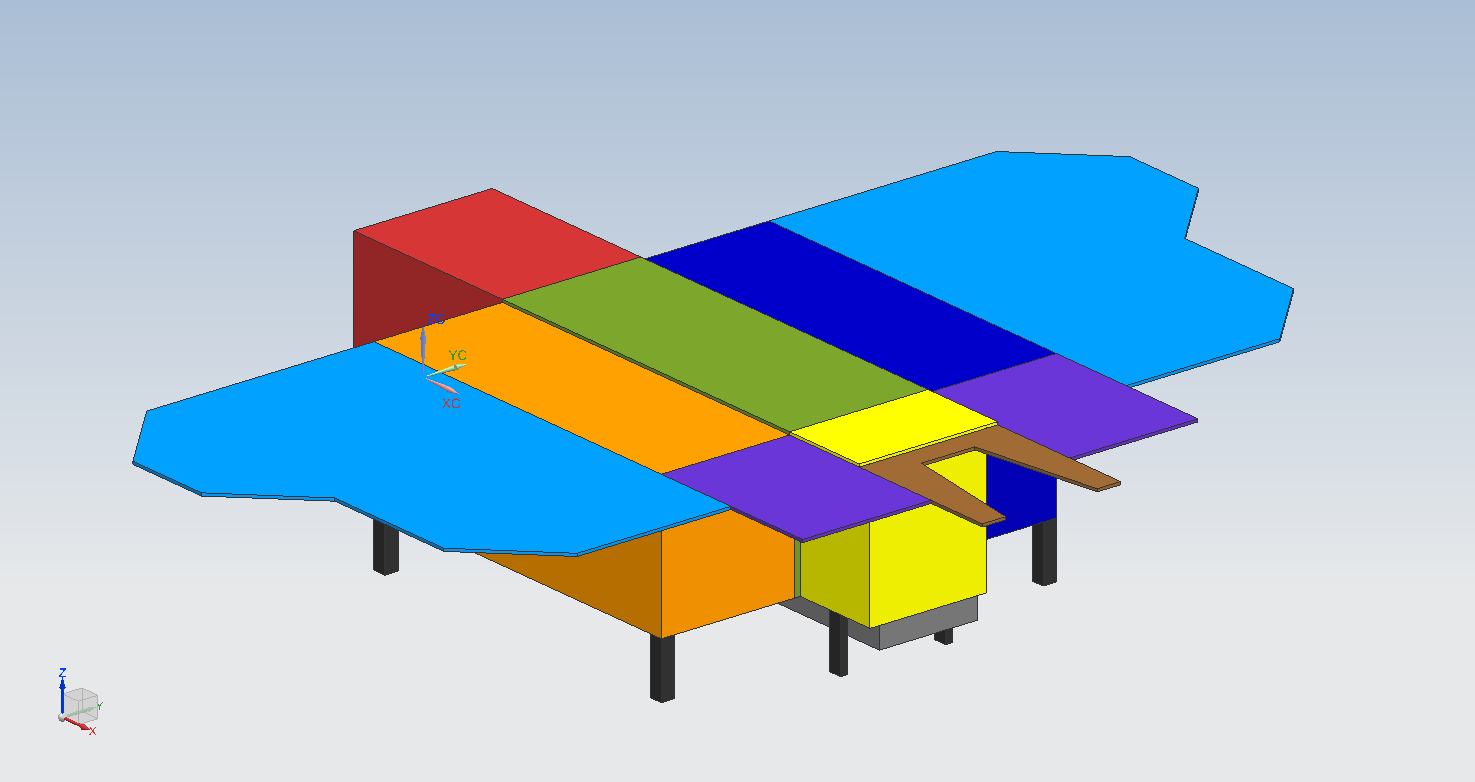
\includegraphics[width=0.5\textwidth]{04_Figures/C.png}
  \captionof{figure}{Modus C}
  \label{Modus C}
\end{center}

\paragraph{Personenlast}\mbox{}\\
Als \emph{Personenlast} werden Lasten verstanden, welche durch Personen im inneren des Solar Butterflys verursacht werden. Im Hauptkörper, sowie in den seitlichen Raumelementen sollen sich total 10 Personen befinden (vgl. Pflichtenheft Personen 4.2.2). Im Kopf, sowie im Heck des Solar Butterflys hat es platzbedingt nur Raum für maximal drei Personen. Das durchschnittliche Gewicht einer Person wird auf 80 kg geschätzt.\\
Die Personenlasten \emph{1.1} bis \emph{1.6} ergeben sich aus der Masse von 10 Personen à 80 kg. Es wird jeweils vereinfacht angenommen, dass sich alle Personen an einem Punkt befinden, wie dies in der Abbildung \ref{Boden} dargestellt ist. Diese Lasten werden entsprechend als Vektorlasten im FEM-Modell eingeleitet. Die Personenlasten \emph{1.7} und \emph{1.8}, welche sich aus den Belastungen von 3 Personen ergeben, werden als Streckenlasten eingeleitet.

\begin{center}
  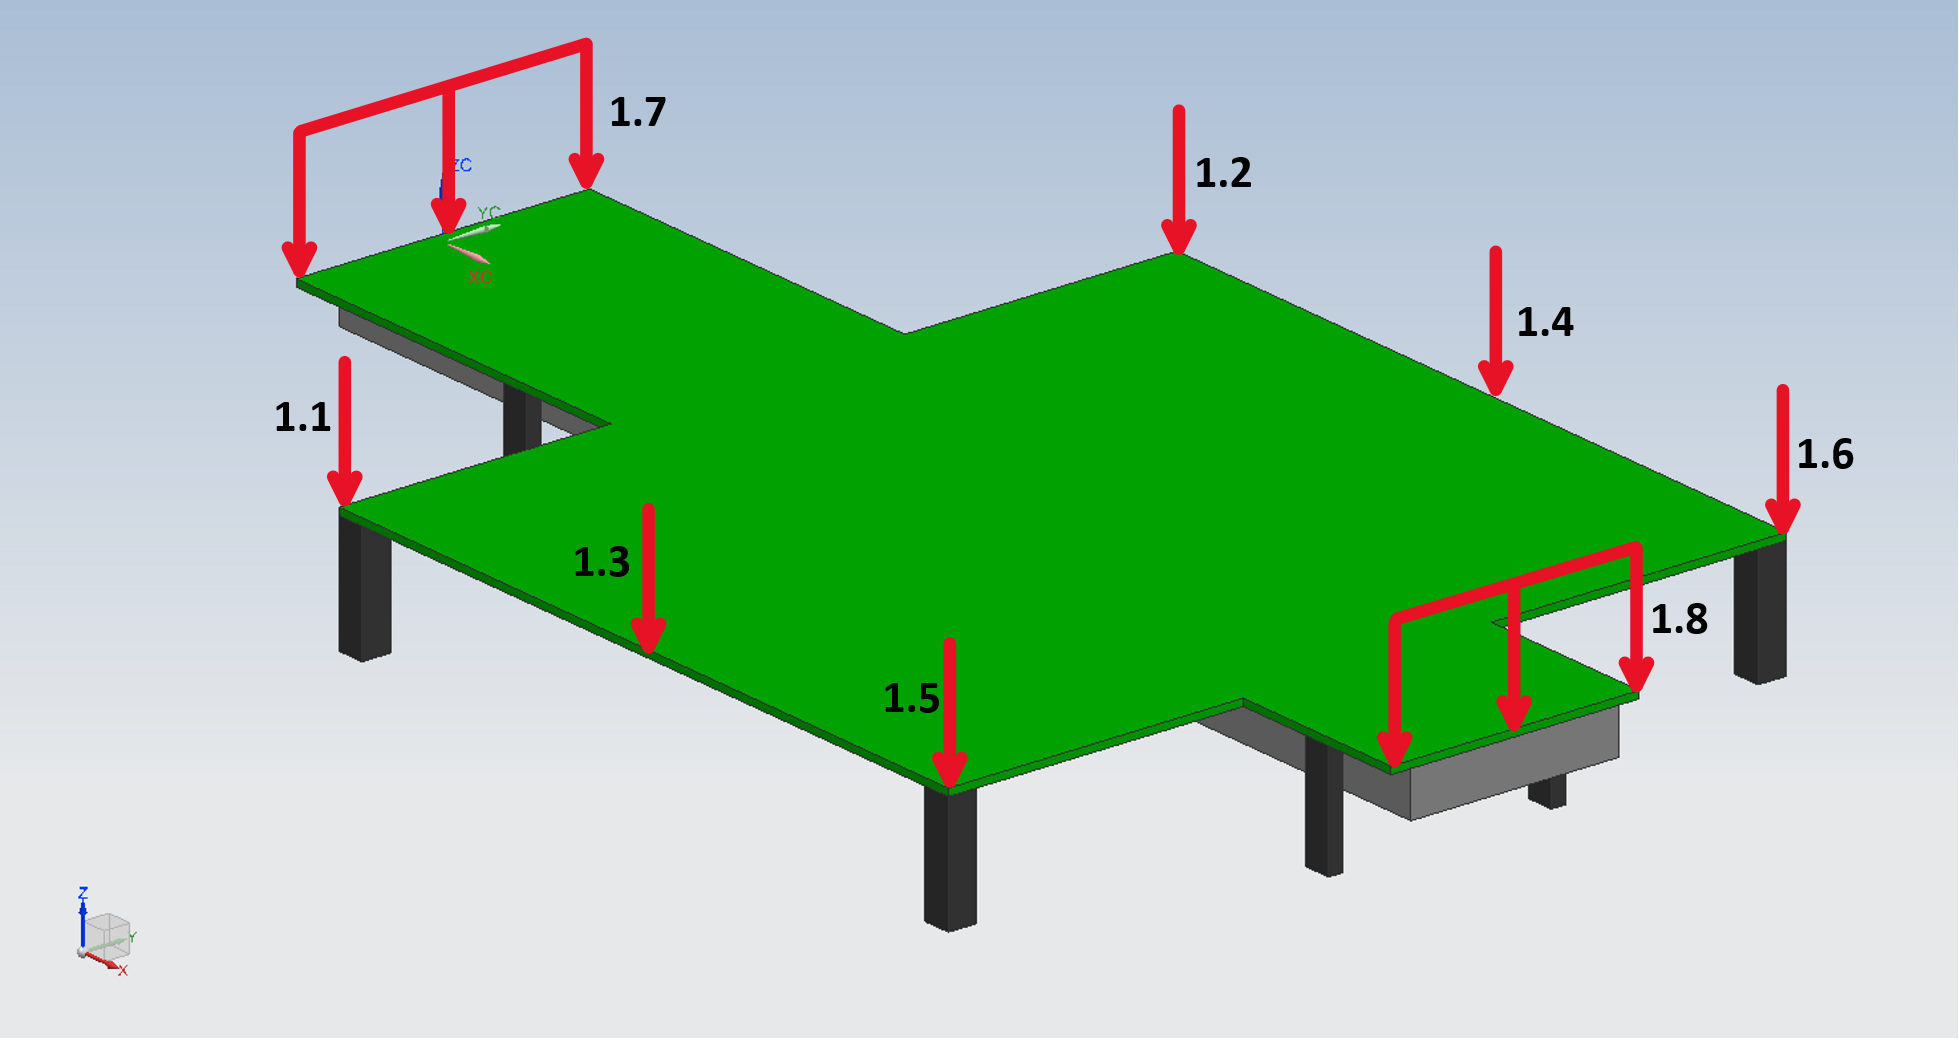
\includegraphics[width=0.8\textwidth]{04_Figures/BodenMitLasten.png}
  \captionof{figure}{Visualisierung der Personenlasten}
  \label{Boden}
\end{center}

Die Fälle, dass Personen in der Mitte eines Raumelementes stehen, werden im Lastenheft nicht aufgeführt, da davon ausgegangen wird, dass diese Fälle für die globalen Lastpfade kein Extrem darstellt. Diese Fälle werden jedoch spezifisch in der Auslegung der Bodenplatten im Kapitel \ref{Boden} berücksichtigt.\\
Die \emph{Ungenauigkeit} sowie die \emph{Auswirkungen} der Personenlasten werden mit den Werten 0.1 und 10 als gering eingeschätzt.

\paragraph{Neigung}\mbox{}\\
Die Lastfälle der Neigung im Modus \emph{C} sind identisch mit jenen des Modus \emph{B}.
% Der Solar Butterfly wird für eine maximale Neigung des Bodens im geparkten Zustand von 5° ausgelegt. Entsprechend wird die Neigung, analog zum den Lastfällen der Neigung im Modus \emph{B}, als Lastfall definiert.\\
% Die \emph{Ungenauigkeit} und die \emph{Auswirkungen} der Lastfälle der Neigung wird mit den Werten 0.1 und 10 ebenfalls als gering eingeschätzt.
% \begin{description}
%   \item \textbf{2.1 Neigung längs positiv}\\
%   +5° Neigung des Untergrundes in Fahrtrichtung.
%   \item \textbf{2.2 Neigung längs negativ}\\
%   -5° Neigung des Untergrundes in Fahrtrichtung.
%   \item \textbf{2.3 Neigung quer positiv}\\
%   +5° Neigung des Untergrundes noraml zur Fahrtrichtung. Ansteig befindet sich in Fahrtrichtung rechts.
%   \item \textbf{2.4 Neigung quer negativ}\\
%   -5° Neigung des Untergrundes noraml zur Fahrtrichtung. Ansteig befindet sich in Fahrtrichtung links.
% \end{description}

\paragraph{Mobiliar}\mbox{}\\
Insegsamt werden drei Lastfälle für die Belastung durch Mobiliar definiert (Für jedes Raumelement einen). Die Belastungen, welche durch das Mobiliar mit einer Masse von 50 kg entstehen, werden jeweils als Flächenlast in FEM-Berechnungen eingeleitet.\\
Die \emph{Ungenauigkeit} sowie die \emph{Auswirkungen} der Lastfälle des Mobiliars werden mit den Werten 0.1 und 10 als gering eingeschätzt.

% \begin{description}
%   \item \textbf{3.1 Mobiliar Hauptmodul}\\
%   Die Flächenlast, welche sich aus den 50 kg Mobiliar ergibt, wird im Boden des Hauptmoduls eingeleitet.
%   \item \textbf{3.2 Mobiliar Seitenteil links}\\
%   Die Flächenlast, welche sich aus den 50 kg Mobiliar ergibt, wird im Boden des linken Seitenmoduls eingeleitet.
%   \item \textbf{3.2 Mobiliar Seitenteil rechts}\\
%   Die Flächenlast, welche sich aus den 50 kg Mobiliar ergibt, wird im Boden des rechten Seitenmoduls eingeleitet.
% \end{description}

\paragraph{Windlasten}\mbox{}\\
Als Windlasten im Modus \emph{C} werden die gemässigten Windlasten des Modus \emph{B}, welche aus Windgeschiwndigkeiten von rund 70 km/h hervorgehen, übernommen.
% Panelen werden auf Beaufort 8 ausgelegt:\\
% Ungenauigkeit: 0.2, Auswirkungen: 20
% \begin{description}
%   \item \textbf{4.1 Wind von links}\\ Der Winddruck von $282 \; Pa$ wirkt auf die, in Fahrtrichtung gesehen, linke Seite des Solar Butterfly.
%   \item \textbf{4.2 Wind von rechts}\\ Der Winddruck von $282 \; Pa$ wirkt auf die, in Fahrtrichtung gesehen, rechte Seite des Solar Butterfly.
% \end{description}


%=============================================================================
%                                 Modus A
%=============================================================================
\begin{landscape}% Landscape page
  \centering % Center table
  \captionof{table}{Lastfälle Modus A}% Add 'table' caption
  \begin{tabularx}{\linewidth}{llcXccc}
    \multicolumn{7}{l}{\LARGE{Modus A: Fahren}}\\
    \thickhline
    Nr. & Bezeichnung & Belastung & Einleitung / Richtung & Uns. & Ausw. & Risiko\\
    \hline
    \multicolumn{7}{l}{\textbf{Beschleunigungen}}\\
    \thickhline
    1.1 & Vertikale Beschleunigung         & $\pm$ 1.5 g           & Beschleunigung in vertikaler Richtung & 0.4 & 50 & 20\\
    1.2 & Longitudinale Beschl. - Positiv  & 0.2 g                 & Beschleunigung in Fahrtrichtung & 0.2 & 20 & 4\\
    1.3 & Longitudinale Beschl. - Negativ  & 0.7 g                 & Verzögerung in Fahrtrichtung & 0.2 & 30 & 6\\
    1.4 & Laterale Beschleunigung          & $\pm$ 0.8 g           & Beschleunigung horizontal und normal zur Fahrtrichtung & 0.1 & 70 & 7\\
    1.5 & Rotatorische Beschleunigung      & 4.4 $\frac{rad}{s^2}$ & Rotatorische Beschleunigung um den Vektor der Fahrtrichtung auf Höhe des Bodens & 0.3 & 60 & 18\\

    \multicolumn{7}{l}{\textbf{Windlasten}}\\
    \thickhline
    2.1 & Wind von links & 532 $Pa$ & Der Winddruck von 532 $Pa$ wirkt auf die, in Fahrtrichtung gesehen, linke Seite des Solar Butterfly. %Diese Windlast entsteht aufgrund von Winden der Stufe 10 auf der Beaufort-Skala (Schwerer Sturm: 102.2 $frac{km}{h}$ Windgeschwindigkeit)
    & 0.4 & 10 & 4\\
    2.2 & Wind von rechts & 532 $Pa$ & Der Winddruck von 532 $Pa$ wirkt auf die, in Fahrtrichtung gesehen, rechte Seite des Solar Butterfly. %Diese Windlast entsteht aufgrund von Winden der Stufe 10 auf der Beaufort-Skala (Schwerer Sturm: 102.2 $frac{km}{h}$ Windgeschwindigkeit)
    & 0.4 & 10 & 4\\

    \multicolumn{7}{l}{\textbf{Belastung durch geneigte Strassen}}\\
    \thickhline
    3.1	& Neigung längs positiv & $+10$° & 10° Neigung des Untergrundes in Fahrtrichtung. Anstieg befindet sich vor dem Fahrzeug. & 0.1 & 10 & 1\\
    3.2	& Neigung längs negativ & $-10$° & -10° Neigung des Untergrundes in Fahrtrichtung. Anstieg befindet sich hinter dem Fahrzeug. & 0.1 & 10 & 1\\
    3.3	& Neigung quer positiv  &$+10$° & 10° Neigung des Untergrundes normal zur Fahrtrichtung. Anstieg befindet sich in Fahrtrichtung rechts. & 0.1 & 10 & 1\\
    3.4	& Neigung quer negativ  &$-10$° & -10° Neigung des Untergrundes normal zur Fahrtrichtung. Anstieg befindet sich in Fahrtrichtung links. & 0.1 & 10 & 1\\

    % \multicolumn{7}{l}{\textbf{Belastung durch verstautes Mobiliar}}\\
    % \thickhline
    % 4.1 & Mobiliar Verstaut & 50 kg & Masse wird im FEM modelliert & 0.4 & 20 & 8\\
    \thickhline
  \end{tabularx}
  \label{Lastenheft A}
\end{landscape}

%=============================================================================
%                                 Modus B
%=============================================================================
\begin{landscape}% Landscape page
  \centering % Center table
  \captionof{table}{Lastfälle Modus B}% Add 'table' caption
  \begin{tabularx}{\linewidth}{llcXccc}
    \multicolumn{7}{l}{\LARGE{Modus B: Ausfahren}}\\
    \thickhline
    Nr. & Bezeichnung & Belastung & Einleitung / Richtung & Uns. & Ausw. & Risiko\\
    \hline
    \multicolumn{7}{l}{\textbf{Windlasten}}\\
    \thickhline
    1.1 & Wind extrem links   & $898 \; Pa$ & Der Winddruck von 898 $\; Pa$ wirkt auf die, in Fahrtrichtung gesehen, linke Seite des Solar Butterfly. %Diese Windlast entsteht aufgrund von Winden der Stufe 12 auf der Beaufort-Skala (Orkan: 132.8 $\frac{km}{h}$ Windgeschwindigkeit)
    & 0.4 & 20 & 8\\
    1.2 & Wind extrem rechts  & $898 \; Pa$ & Der Winddruck von 898 $\; Pa$ wirkt auf die, in Fahrtrichtung gesehen, rechte Seite des Solar Butterfly. %Diese Windlast entsteht aufgrund von Winden der Stufe 12 auf der Beaufort-Skala (Orkan: 132.8 $\frac{km}{h}$ Windgeschwindigkeit)
    & 0.4 & 20 & 8\\
    1.3 & Wind von links      & $532 \; Pa$ & Der Winddruck von 532 $\; Pa$ wirkt auf die, in Fahrtrichtung gesehen, linke Seite des Solar Butterfly. %Diese Windlast entsteht aufgrund von Winden der Stufe 10 auf der Beaufort-Skala (Schwerer Sturm: 102.2 $\frac{km}{h}$ Windgeschwindigkeit)
    & 0.4 & 10 & 4\\
    1.4 & Wind von rechts     & $532 \; Pa$ & Der Winddruck von 532 $\; Pa$ wirkt auf die, in Fahrtrichtung gesehen, rechte Seite des Solar Butterfly. %Diese Windlast entsteht aufgrund von Winden der Stufe 10 auf der Beaufort-Skala (Schwerer Sturm: 102.2 $\frac{km}{h}$ Windgeschwindigkeit)
    & 0.4 & 10 & 4\\
    \\[\lineHeightTable]

    \multicolumn{7}{l}{\textbf{Belastung durch geneigten Boden}}\\
    \thickhline
    2.1	& Neigung längs positiv & $+5$° & 5° Neigung des Untergrundes in Fahrtrichtung. Anstieg befindet sich vor dem Fahrzeug. & 0.1 & 10 & 1\\
    2.2	& Neigung längs negativ & $-5$° & -5° Neigung des Untergrundes in Fahrtrichtung. Anstieg befindet sich hinter dem Fahrzeug. & 0.1 & 10 & 1\\
    2.3	& Neigung quer positiv  & $+5$° & 5° Neigung des Untergrundes noraml zur Fahrtrichtung. Ansteig befindet sich in Fahrtrichtung rechts. & 0.1 & 10 & 1\\
    2.4	& Neigung quer negativ  & $-5$° & -5° Neigung des Untergrundes noraml zur Fahrtrichtung. Ansteig befindet sich in Fahrtrichtung links. & 0.1 & 10 & 1\\

    % \multicolumn{7}{l}{\textbf{Belastung durch  Mobiliar}}\\
    % \thickhline
    % 3.1 & Mobiliar Verstaut & 50 kg & Masse wird im FEM modelliert & 0.1 & 10 & 8\\
    \thickhline
  \end{tabularx}
\end{landscape}

%=============================================================================
%                                 Modus C
%=============================================================================
\begin{landscape}% Landscape page
    \centering % Center table
    \begin{longtable}{llc L{10cm} ccc}
      \caption{Lastfälle Modus C}\\
        \multicolumn{7}{l}{\LARGE{Modus C: Stehend}}\\
        \thickhline
        Nr. & Bezeichnung & Belastung & Einleitung / Richtung & Uns. & Ausw. & Risiko\\
        \hline
        \multicolumn{7}{l}{\textbf{Belastung durch Personen}}\\
        \thickhline
        1.1 &	Personenlast vorne Li	  & 800 kg &	Vordere linke Ecke des linken ausfahrbaren Raumelementes	            & 0.2 &	20 & 4\\
        1.2 &	Personenlast vorne Re	  & 800 kg &	Vordere rechte Ecke des rechten ausfahrbaren Raumelementes	          & 0.2 &	20 & 4\\
        1.3 &	Personenlast mitte Li	  & 800 kg &	In der Mitte der Äussere Kante des linken ausfahrbaren Raumelementes  & 0.2 &	20 & 4\\
        1.4 &	Personenlast mitte Re	  & 800 kg &	In der Mitte der Äussere Kante des rechten ausfahrbaren Raumelementes & 0.2 &	20 & 4\\
        1.5 &	Personenlast hinten Li	& 800 kg &	Hintere linke Ecke des linken ausfahrbaren Raumelementes	            & 0.2 &	20 & 4\\
        1.6 &	Personenlast hinten Re	& 800 kg &	Hintere rechte Ecke des rechten ausfahrbaren Raumelementes	          & 0.2 &	20 & 4\\
        1.7 &	Personenlast Küche	    & 240 kg  &	Streckenlast auf vorderste Kante	                                      & 0.1 &	20 & 2\\
        1.8 &	Personenlast Bad	      & 240 kg  &	Streckenlast auf hinterste Kante	                                    & 0.1 &	20 & 2\\

        \multicolumn{7}{l}{\textbf{Belastung durch geneigten Boden}}\\
        \thickhline
        2.1	& Neigung längs positiv & $+5$° & 5° Neigung des Untergrundes in Fahrtrichtung. Der Anstieg befindet sich vor dem Fahrzeug. & 0.1 & 10 & 1\\
        2.2	& Neigung längs negativ & $-5$° & -5° Neigung des Untergrundes in Fahrtrichtung. Der Anstieg befindet sich hinter dem Fahrzeug. & 0.1 & 10 & 1\\
        2.3	& Neigung quer positiv  & $+5$° & 5° Neigung des Untergrundes normal zur Fahrtrichtung. Der Anstieg befindet sich in Fahrtrichtung rechts. & 0.1 & 10 & 1\\
        2.4	& Neigung quer negativ  & $-5$° & -5° Neigung des Untergrundes normal zur Fahrtrichtung. Der Anstieg befindet sich in Fahrtrichtung links. & 0.1 & 10 & 1\\

        \multicolumn{7}{l}{\textbf{Belastung durch  Mobiliar}}\\
        \thickhline
        3.1	& Mobiliar Mittleres Raumelement	& 50 kg &	Einleitung als Flächenlast im mittleren Raumelement &	0.1 &	10 &	1\\
        3.2	& Mobiliar Raumelement links	    & 50 kg &	Einleitung als Flächenlast im linken ausfahrbaren Raumelement & 0.1 & 10 &	1\\
        3.3	& Mobiliar Raumelement rechts	    & 50 kg &	Einleitung als Flächenlast im rechten ausfahrbaren Raumelement &	0.1 &	10 &	1\\

        \multicolumn{7}{l}{\textbf{Windlasten}}\\
        \thickhline
        4.1 & Wind von links  & $532 \; Pa$ & Der Winddruck von 532 $Pa$ wirkt auf die, in Fahrtrichtung gesehen, linke Seite des Solar Butterfly & 0.4 & 10 & 4\\
        4.2 & Wind von rechts & $532 \; Pa$ & Der Winddruck von 532 $Pa$ wirkt auf die, in Fahrtrichtung gesehen, rechte Seite des Solar Butterfly & 0.4 & 10 & 4\\
        \thickhline
    \end{longtable}
\end{landscape}
\clearpage% Flush page

\newpage

  \section{Komponenten und Verbindungen}
In diesem Kapitel wird beschrieben, wie der Solar Butterfly aufgebaut ist. Es werden verschiedene Komponenten eingeführt und analysiert wie diese Komponenten miteinander Verbunden sind und welche Kräfte die Verbindungen übertragen müssen.\\
Weiter wird beschrieben, wie der SB vereinfacht betrachtet wird (Biegebalken) in zwei Moden. (A und C)

\subsection{Komponenten}
bla bla

\paragraph{Hauptkörper}
Ganzer Körper als einen Kasten betrachten
\begin{description}
  \item \textbf{Chassis}\\
  Idealisierung: Beam
  \item \textbf{Boden}\\
  Auslegung: Biegebalken
  Idealisierung: Schalenkörper\\
  \item \textbf{Stützen A und B}\\
  Auslegung: Schubwand mit Türe\\
  Profile nehmen Kräfte auf, geben diese Jedoch an die Schubwand weiter\\
  \item \textbf{Dach}\\
  Panelen: Schubfläche\\
  Dach an sich: Biegebalken (Durch eigengewicht)
  Im Modus \emph{C} Kräfte auf nehmen durch Verriegelung der Seitenwände\\
  \item \textbf{}
\end{description}

\paragraph{Seitenmodul}
\begin{description}
  \item \textbf{Boden}\\
  Biegebalken und Schubfläche
  \item \textbf{Seitenwand}\\
  Modus A: Schubwand\\
  Modus C: Keine
  \item \textbf{Ausfahrmechanismus (Scharniere)}\\
  Wand: Schubwand
  \item \textbf{}\\
  \item \textbf{}\\
\end{description}

  \section{FEM}
  Wie ist das FEM aufgesetzt und welchen Zweck erfüllt es?
  \section{Auslegung und Design}
  Hier werden Komponenten und Baugruppen ausgelegt

% ==================== Backmatter ====================
  \part{Anhang}
  \appendix
  \section{Quellenverzeichnis}

\renewcommand\refname{\vskip -1cm}
\bibliography{03_Backmatter/mybib}
\bibliographystyle{ieeetr}

  \section{Abbildungsverzeichnis}
\renewcommand\listfigurename{}
\vspace*{-1cm}
\listoffigures

  \section{Tabellenverzeichnis}
\renewcommand\listtablename{}
\vspace*{-1cm}
\listoftables
\newpage

  \section{Lastenheft}
  \subsection{Berechnung der Vertikalen Beschleunigung}
  Die Position des Rades während dem Überfahren der Bremsschwelle ist gegeben durch folgenden Zusammenhang:
  \begin{equation}
    x_r^n = h \cdot sin\left(\pi \cdot \frac{n \cdot \Delta t \cdot v}{l}\right)
  \end{equation}
  $l$ steht dabei für die Länge, und h für die Höhe der Bremsschwelle. $v$ für die Geschwindigkeit des Solar Butterflys beim Überfahren, $n$ für den Zeitschritt und $\Delta t$ für die Zeitinkrementierung pro Berechnungsschritt.\\

  Um die Beschleunigung des Solar Butterflys zu berechnen, wird in einem ersten Schritt dessen Position zum Zeitpunk $n$ $x_{SB}^n$ aus der vorangehenden Situation berechnet.
  \begin{equation}
    x_{SB}^n = x_{SB}^{(n-1)} + v^{(n-1)} \cdot \Delta t
  \end{equation}

  Als nächstes wird der Federweg $s^n$, sowie die Änderungsrate des Federwegs $v_s^n$ zum Zeitpunkt $n$ aus den Positionen des Rades $r_x^n$ und des Solar Butterflys $x_{SB}^n$ berechnet.
  \begin{equation}
    s^n = x_r^n - x_{SB}^n
  \end{equation}
  \begin{equation}
    v_s^n = \frac{s^n - s^{(n-1)}}{\Delta t}
  \end{equation}

  Die Beschleunigung des Solar Butterfly ergibt sich dann zu:\\
  \begin{equation}
    a_{SB}^n = \frac{k \cdot s^n + d \cdot v_s^n}{m}
  \end{equation}

  Wobei $k$ für die Federkonstante und $d$ für die Dämpfungskonstante stehen.
  Die aus der Beschleunigung des Solar Butterfly resultierende neue Geschwindigkeit, kann wie folgt berechnet werden.
  \begin{equation}
    v^n = v^{(n-1)} + a_{SB}^n \cdot \Delta t
  \end{equation}



\section{FEM}

\subsection{FEM Ergebnisse}
  \label{FEM Ergebnisse}

  \subsubsection{FEM-Ergebnis - Lastfall 1.1 Vertikale Beschleunigung}
  \begin{table}[H]
  \centering
  \begin{tabular}{lcccccc}
  Grösse	&	Einheit	&	x	&	y	&	z	&	Total	&	Berechnet	\\	\hline
  \multicolumn{5}{l}{\textbf{Lagerreaktionen}}									&		&		\\	\thickhline
  Deichsel	&	N	&	0	&	3193	&	0	&	3193	&	-1028	(y) \\
  Chassis Links	&	N	&	0	&	35171	&	6733	&	35810	&	37300 (y)	\\
  Chassis Rechts	&	N	&	0	&	35171	&	-6733	&	35810	&	37300 (y)	\\	\hline	\\
  \multicolumn{5}{l}{\textbf{Chassis}}									&		&		\\	\thickhline
  Axialkraft	&	N	&		&		&		&	-50730	&	-44518	\\
  Querkraft	&	N	&		&		&		&	17003	&	19079	\footnotemark \\
  Biegemoment	&	kNmm	&		&		&		&	16980	&		\\	\hline	\\
  \multicolumn{5}{l}{\textbf{Dach}}									&		&		\\	\thickhline
  Axialkraft	&	N	&		&		&		&	2879	&	14840	\\
  Querkraft	&	N	&		&		&		&	108	&		\\
  Biegemoment	&	kNmm	&		&		&		&	42	&		\\	\hline	\\
  \multicolumn{5}{l}{\textbf{Träger A und B}}													\\	\thickhline
  Axialkraft	&	N	&		&		&		&	-10904	&		\\
  Querkraft	&	N	&		&		&		&	1293	&		\\
  Biegemoment	&	kNmm	&		&		&		&	327	&		\\	\hline	\\
  \multicolumn{5}{l}{\textbf{Kontaktreaktion: Chassis - Träger A und B}}									&		&		\\	\thickhline
   Axialkraft A	&	N	&	-620	&	12931	&	-218	&	12948	&		\\
  Biegemoment A	&	kNmm	&	-4602	&	-179	&	341	&	4618	&		\\
  Axialkraft B	&	N	&	2464	&	15784	&	713	&	15991	&		\\
  Biegemoment B	&	kNmm	&	-5610	&	851	&	-346	&	5685	&		\\	\hline	\\
  \multicolumn{5}{l}{\textbf{Kontaktreaktion: Chassis - Boden}}									&		&		\\	\thickhline
  Normalkraft (Zug)	&	N	&		&		&		&	883	&		\\
  Schubkraft (xz-Ebene)	&	N	&		&		&		&	9933	&		\\	\hline
  \end{tabular}
  \caption{Resultate der FEM-Simulation des Lastafalles der vertikalen Beschleunigung}
  \label{tab:FEM 1.1}
  \end{table}
  \footnotetext[2]{Unter der Annahme, dass nur das Chassis Querkräfte aufnimmt. Die Kraft von 19 kN ergibt sich aus der Halbierung der globalen Querkraft aus der Berechnung im Kapitel \ref{1.1 Vertikale Beschleunigung}.}

  \subsubsection{FEM-Ergebnis - Lastfall 1.3 Longitudinale Beschleunigung negativ}
  \begin{table}[H]
  \centering
  \begin{tabular}{lcccccc}
  Grösse	&	Einheit	&	x	&	y	&	z	&	Total	&	Berechnet	\\	\hline
  \multicolumn{5}{l}{\textbf{Lagerreaktionen}}									&		&		\\	\thickhline
  Deichsel	&	N	&	-20611	&	-3050	&	0	&	20835	&	206000 (x)	\\
  Chassis Links	&	N	&	0	&	1525	&	515	&	1610	&		\\
  Chassis Rechts	&	N	&	0	&	1525	&	-515	&	1610	&		\\	\hline	\\
  \multicolumn{5}{l}{\textbf{Chassis}}									&		&		\\	\thickhline
  Axialkraft	&	N	&		&		&		&	6080	&		\\
  Querkraft	&	N	&		&		&		&	1319	&		\\
  Biegemoment	&	kNmm	&		&		&		&	2601	&		\\	\hline	\\
  \multicolumn{5}{l}{\textbf{Dach}}									&		&		\\	\thickhline
  Axialkraft	&	N	&		&		&		&	553	&		\\
  Querkraft	&	N	&		&		&		&	8	&		\\
  Biegemoment	&	kNmm	&		&		&		&	2	&		\\	\hline	\\
  \multicolumn{5}{l}{\textbf{Träger A und B}}													\\	\thickhline
  Axialkraft	&	N	&		&		&		&	-1562	&		\\
  Querkraft	&	N	&		&		&		&	56	&		\\
  Biegemoment	&	kNmm	&		&		&		&	17	&		\\	\hline	\\
  \multicolumn{5}{l}{\textbf{Kontaktreaktion: Chassis - Träger A und B}}									&		&		\\	\thickhline
   Axialkraft A	&	N	&	-56	&	2084	&	325	&	2110	&		\\
  Biegemoment A	&	kNmm	&	-734	&	-19	&	2	&	734	&		\\
  Axialkraft B	&	N	&	98	&	667	&	80	&	679	&		\\
  Biegemoment B	&	kNmm	&	-236	&	34	&	-14	&	238	&		\\	\hline	\\
  \multicolumn{5}{l}{\textbf{Kontaktreaktion: Chassis - Boden}}									&		&		\\	\thickhline
  Normalkraft (Zug)	&	N	&		&		&		&	35	&		\\
  Schubkraft (xz-Ebene)	&	N	&		&		&		&	1733	&		\\	\hline
  \end{tabular}
  \caption{Resultate der FEM-Simulation des Lastafalles der longitudinalen Beschleunigung}
  \label{tab:FEM 1.3}
  \end{table}


  \subsubsection{FEM-Ergebnis - Lastfall 1.4 laterale Beschleunigung}
  \begin{table}[H]
  \centering
  \begin{tabular}{lcccccc}
  Grösse	&	Einheit	&	x	&	y	&	z	&	Total	&	Berechnet	\\	\hline
  \multicolumn{5}{l}{\textbf{Lagerreaktionen}}									&		&		\\	\thickhline
  Deichsel	&	N	&	0	&	0	&	1023	&	1023	&	-330 (z)	\\
  Chassis Links	&	N	&	0	&	-15008	&	11290	&	18780	&	11900 (z)	\\
  Chassis Rechts	&	N	&	0	&	15008	&	11242	&	18752	&	11900 (z)	\\	\hline	\\
  \multicolumn{5}{l}{\textbf{Chassis}}									&		&		\\	\thickhline
  Axialkraft	&	N	&		&		&		&	-31674	&	-11480	\\
  Querkraft	&	N	&		&		&		&	7163	&	6100	\footnotemark \\
  Biegemoment	&	kNmm	&		&		&		&	6658	&		\\	\hline	\\
  \multicolumn{5}{l}{\textbf{Dach}}									&		&		\\	\thickhline
  Axialkraft	&	N	&		&		&		&	-2560	&	-964	\\
  Querkraft	&	N	&		&		&		&	24	&		\\
  Biegemoment	&	kNmm	&		&		&		&	13	&		\\	\hline	\\
  \multicolumn{5}{l}{\textbf{Träger A und B}}													\\	\thickhline
  Axialkraft	&	N	&		&		&		&	2684	&		\\
  Querkraft	&	N	&		&		&		&	1067	&	470	\\
  Biegemoment	&	kNmm	&		&		&		&	627	&	470	\\	\hline	\\
  \multicolumn{5}{l}{\textbf{Kontaktreaktion: Chassis - Träger A und B}}									&		&		\\	\thickhline
   Axialkraft A	&	N	&	237	&	-3577	&	1729	&	3979	&		\\
  Biegemoment A	&	kNmm	&	1924	&	71	&	-102	&	1928	&		\\
  Axialkraft B	&	N	&	-733	&	-4221	&	1679	&	4602	&		\\
  Biegemoment B	&	kNmm	&	2097	&	-251	&	95	&	2114	&		\\	\hline	\\
  \multicolumn{5}{l}{\textbf{Kontaktreaktion: Chassis - Boden}}									&		&		\\	\thickhline
  Normalkraft (Zug)	&	N	&		&		&		&	1942	&		\\
  Schubkraft (xz-Ebene)	&	N	&		&		&		&	10972	&		\\	\hline
  \end{tabular}
  \caption{Resultate der FEM-Simulation des Lastafalles der lateralen Beschleunigung}
  \label{tab:FEM 1.4}
  \end{table}
  \footnotetext[3]{Unter der Annahme, dass nur das Chassis Querkräfte aufnimmt. Die Kraft von 6.1 kN ergibt sich aus der Halbierung der globalen Querkraft aus der Berechnung im Kapitel \ref{1.4 Laterale Beschleunigung}.}


  \subsubsection{FEM-Ergebnis - Lastfall 1.5 Rotatorische Beschleunigung}
  \begin{table}[H]
  \centering
  \begin{tabular}{lcccccc}
  Grösse	&	Einheit	&	x	&	y	&	z	&	Total	&	Berechnet	\\	\hline
  \multicolumn{5}{l}{\textbf{Lagerreaktionen}}									&		&		\\	\thickhline
  Deichsel	&	N	&	0	&	0	&	804	&	804	&		\\
  Chassis Links	&	N	&	0	&	-23097	&	10913	&	25546	&	-27000 (y)	\footnotemark \\
  Chassis Rechts	&	N	&	0	&	23097	&	10844	&	25516	&	27000 (y)	\\	\hline	\\
  \multicolumn{5}{l}{\textbf{Chassis}}									&		&		\\	\thickhline
  Axialkraft	&	N	&		&		&		&	-44164	&		\\
  Querkraft	&	N	&		&		&		&	10927	&		\\
  Biegemoment	&	kNmm	&		&		&		&	10218	&		\\	\hline	\\
  \multicolumn{5}{l}{\textbf{Dach}}									&		&		\\	\thickhline
  Axialkraft	&	N	&		&		&		&	-3625	&		\\
  Querkraft	&	N	&		&		&		&	32	&		\\
  Biegemoment	&	kNmm	&		&		&		&	19	&		\\	\hline	\\
  \multicolumn{5}{l}{\textbf{Träger A und B}}													\\	\thickhline
  Axialkraft	&	N	&		&		&		&	-4119	&		\\
  Querkraft	&	N	&		&		&		&	1311	&		\\
  Biegemoment	&	kNmm	&		&		&		&	772	&		\\	\hline	\\
  \multicolumn{5}{l}{\textbf{Kontaktreaktion: Chassis - Träger A und B}}									&		&		\\	\thickhline
   Axialkraft A	&	N	&	373	&	-5525	&	2346	&	6014	&		\\
  Biegemoment A	&	kNmm	&	2767	&	112	&	-164	&	2774	&		\\
  Axialkraft B	&	N	&	-1309	&	-6399	&	2221	&	6899	&		\\
  Biegemoment B	&	kNmm	&	2996	&	-452	&	159	&	3034	&		\\	\hline	\\
  \multicolumn{5}{l}{\textbf{Kontaktreaktion: Chassis - Boden}}									&		&		\\	\thickhline
  Normalkraft (Zug)	&	N	&		&		&		&	3118	&		\\
  Schubkraft (xz-Ebene)	&	N	&		&		&		&	10761	&		\\	\hline
  \end{tabular}
  \caption{Resultate der FEM-Simulation des Lastafalles der rotatorischen Beschleunigung}
  \label{tab:FEM 1.5}
  \end{table}
  \footnotetext[4]{Die Kräfte von  $\pm$ 27 kN ergeben sich aus der Halbierung der Kraft F aus der Berechnung im Kapitel \ref{1.5 Rotatorische Beschleunigung}.}
    \newpage

\subsection{Deformationen}
\label{FEM Deformation}
\subsubsection{Deformation - Lastfall 1.1 Vertikale Beschleunigung}
\begin{figure}[H]
  \centering
  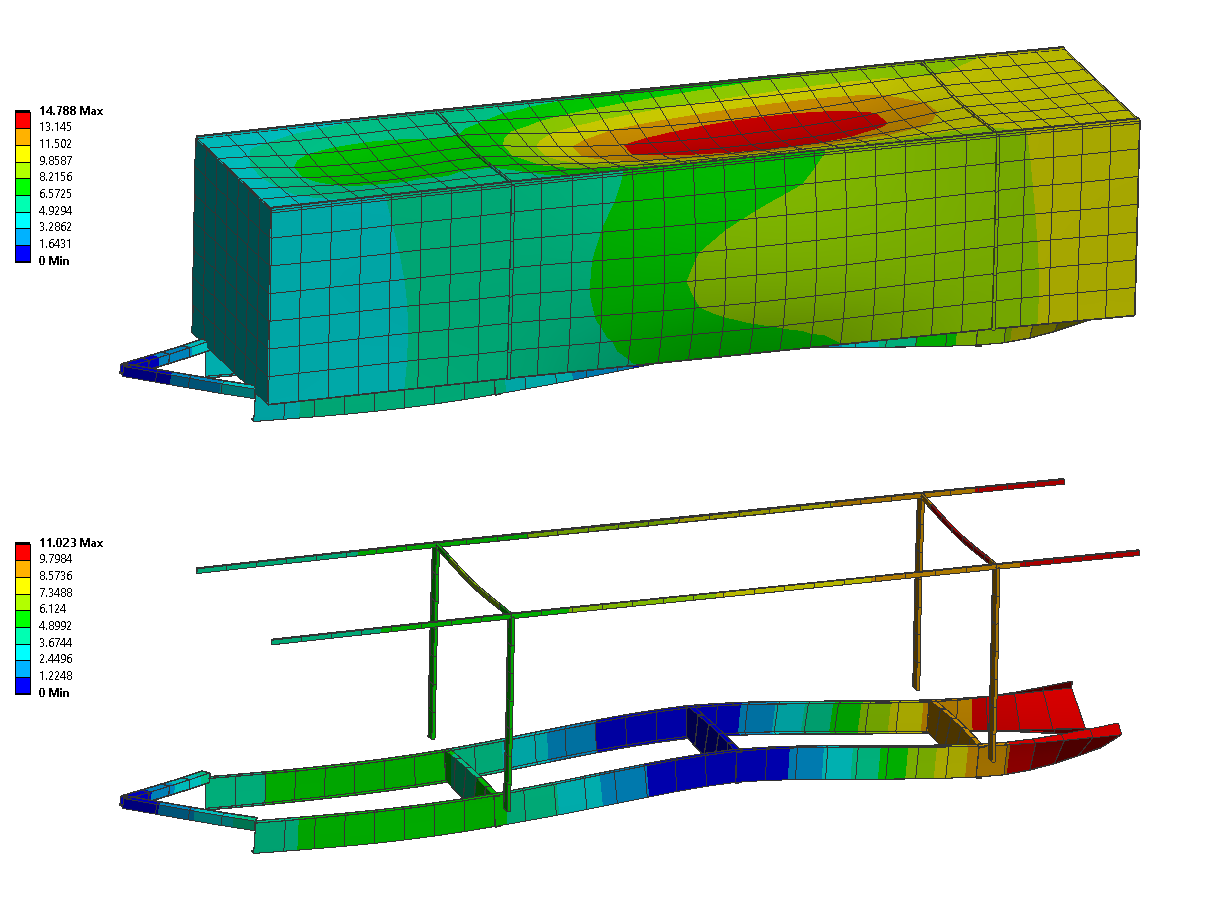
\includegraphics[width=1\linewidth]{04_figures/FEM 1.1.png}
  \caption{Deformation des Solar Butterflys im Lastfall der vertikalen Beschleunigung}
  \label{FEM 1.1}
\end{figure}

\subsubsection{Deformation - Lastfall 1.3 Longitudinale Beschleunigung}
\begin{figure}[H]
  \centering
  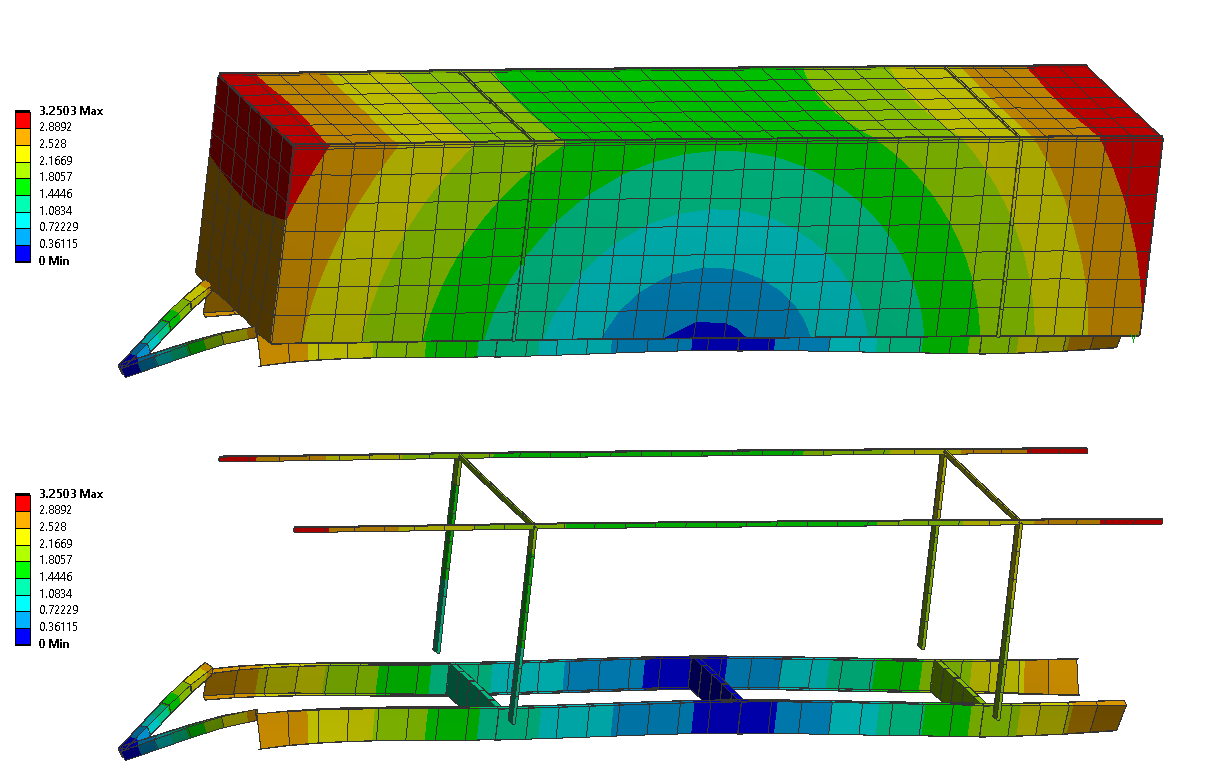
\includegraphics[width=1\linewidth]{04_figures/FEM 1.2.png}
  \caption{Deformation des Solar Butterflys im Lastfall der lateralen Beschleunigung}
  \label{FEM 1.3}
\end{figure}

\subsubsection{Deformation - Lastfall 1.4 Laterale Beschleunigung}
\begin{figure}[H]
  \centering
  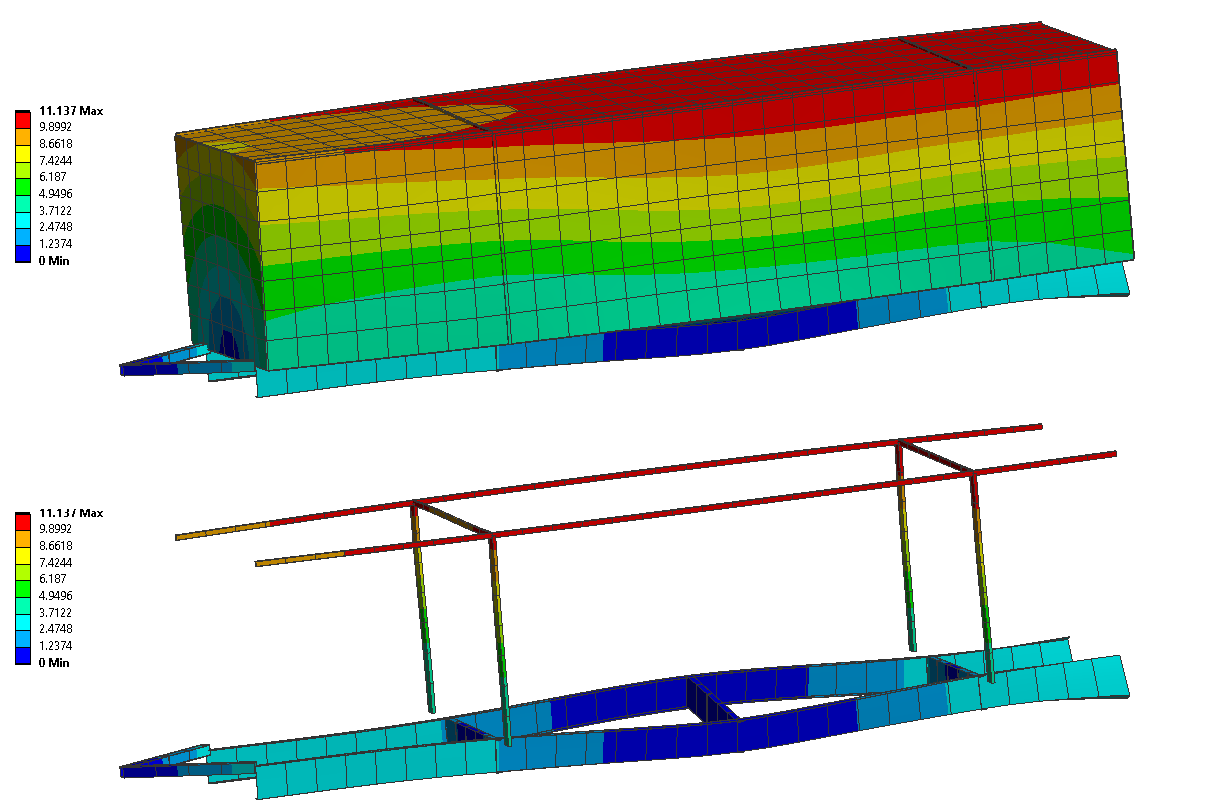
\includegraphics[width=1\linewidth]{04_figures/FEM 1.4.png}
  \caption{Deformation des Solar Butterflys im Lastfall der longitudinalen Beschleunigung}
  \label{FEM 1.4}
\end{figure}

\subsubsection{Deformation - Lastfall 1.5 Rotatorische Beschleunigung}
\begin{figure}[H]
  \centering
  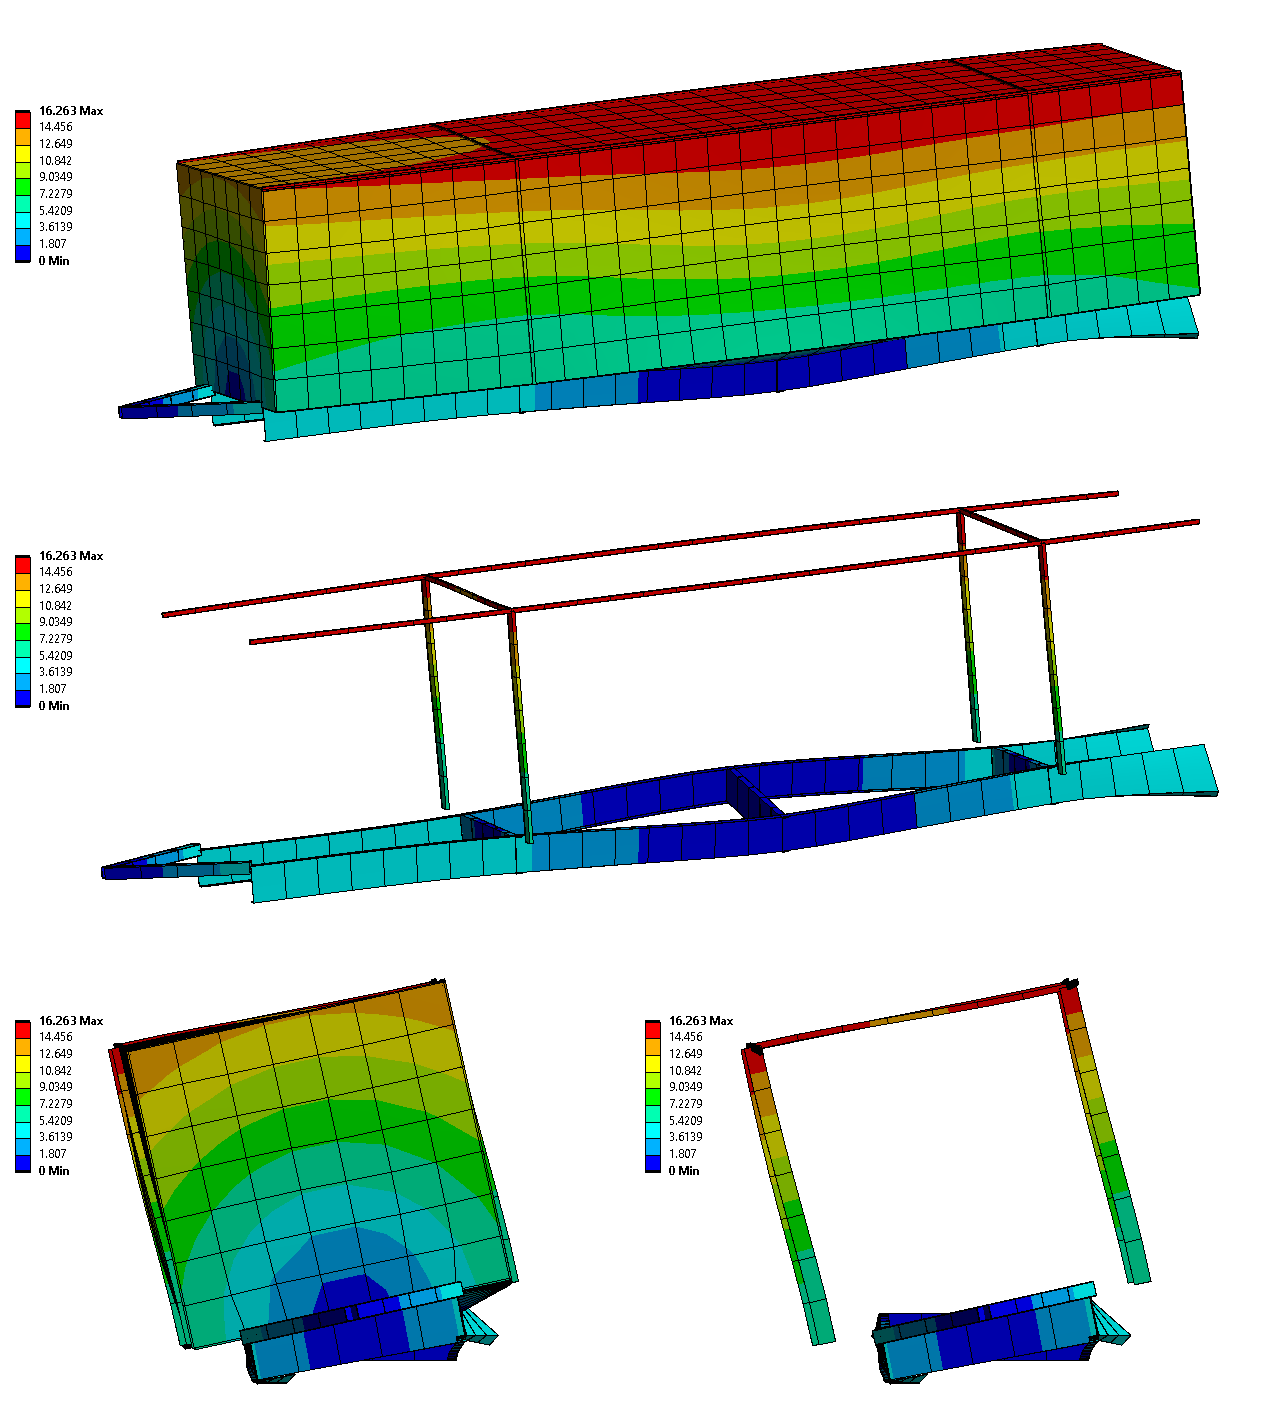
\includegraphics[width=1\linewidth]{04_figures/FEM 1.5.png}
  \caption{Deformation des Solar Butterflys im Lastfall der rotatorischen Beschleunigung}
  \label{FEM 1.5}
\end{figure}
\newpage


  \part{Elektronischer Anhang}
  \appendix
  \section{Bilder des Solar Butterflys}
\label{Bilder des Solar Butterflys}



\section{Dokumente aus fremden Arbeiten}
  \subsection{Anforderungsliste}
  \label{e:Anforderungsliste}
  \subsection{Gewichtsberechnung}
  \label{e:Gewichtsberechnung}




\section{Datenblätter}
  \subsection{Materialien}
  \label{e:Materialien}
    \subsubsection{TDS Airex-T92}
    \label{e:Airex}
    \subsubsection{TDS Sikafles 552-AT}
    \label{e:Sikaflex}

  \subsection{Komponenten}
    \subsubsection{Federkennlinie-Hysterese}
    \label{e:Federkonstante}



\section{Berechnungen}
\label{e:Berechnungen}
  \subsection{Lastenheft - Beschleunigungen}
  \label{e:Lastenheft}
  \subsection{Handrechnungen}
  \label{e:Handrechnungen}
  \subsection{Dimensionierung}
  \label{e:Dimensionierung}
  \subsection{Dimensionierung Solarpanelen}
  \label{e:Solarpanelen}



\section{FEM}
  \subsection{FEM-Modell - Solarpanelen}
  \label{e:Panelen}
  \subsection{FEM-Modell - Solar Butterfly Global}
  \label{e:Globales FEM}
  \subsection{FEM Auswertung}
  \label{e:FEM Auswertung}

\end{document}
